\documentclass{swfuthesis}

\usepackage{biolinum}
\newcommand\Ctrl[1]{\LKeyCtrlX{#1}} % for Ctrl-u Ctrl-l

\graphicspath{{./image}}

\addbibresource{thesis.bib} % 参照教程自己去写一个.bib文件

\swfusetup{%
  Title={基于Linux的操作系统研究}, % 论文标题
  Author={杨鑫}, % 作者姓名
  ID={20211159013},%
  Signature={
\includegraphics[width=6em]{yangxin.pdf}},%
  enTitle={Research on Operating System based on Linux},%
  enAuthor={YangXin}, % 作者姓名(英文)
  Advisor={王晓林(讲师)}, % 指导教师姓名(职称)
  Reviewer={},
  Year={\the\year},
  Month={\the\month},
  Date={\the\day},
  Major={计算机科学与技术专业}, %专业名称(比如 电子信息工程专业)
}

\begin{document}

\maketitle
\frontmatter

\begin{abstract} % 摘要
  本文研究的是基于Linux的操作系统。首先介绍了Linux的发展历程及其特点,包括开源、自由、可定
  制等。接着详细介绍了Linux操作系统的内核结构和系统调用,解释了Linux的开机过程、中断、进程
  管理、文件系统。

  在学习了Linux操作系统的基础后,本文在此基础上实现了一个简单的操作系统。该
  操作系统采用汇编语言与C语言编写,实现了简单的进程管理、文件系统和一个简单
  的Shell. 在实现过程中,本文详细阐述了操作系统的设计思路、算法实现和关键技术,包括进程调
  度算法、中断处理算法、文件系统实现和shell的一些基本功能应用。
\end{abstract}

\begin{keyword} % 关键词
Boot; Loader; GDT; Kernel; 中断; 进程调度; Shell;
\end{keyword}

\begin{EAbstract}
  This paper studies the operating system based on Linux. Firstly, it introduces the development history and characteristics of Linux, including open source, freedom,
  System etc. Next, the internal structure and system adjustment of the Linux operating system are introduced in detail, and the boot process, interruption, and process of Linux are explained.
  Management, file system.

  After learning the basis of the Linux operating system, this article implements a simple operating system on this basis.
  The operating system is based on the Linux kernel, written in assembly language and C language, and realizes simple program management, file system and a simple single
  shell. In the actual process, this paper describes in detail the design ideas, algorithm reality and key technologies of the operating system, including
  Some basic functional applications of calculation method, interrupt processing method, file system implementation and shell.
\end{EAbstract}
\begin{EKeyword}
Boot; Loader; GDT; Kernel; Interrupt; Process Scheduling; Shell;  
\end{EKeyword}

\tableofcontents     % 目录
% \listoffigures       % 插图目录,可以没有
% \listoftables        % 表格目录,可以没有
\cleardoublepage % keep this line
%\pagenumbering{arabic}

\mainmatter

% 参考教程,在chapters目录中单独写各章(ch1.tex, ch2.tex...)
\chapter{绪论}
\section{背景及意义}
\label{sec:env}

\subsection{背景}
%\footnote{参考自\url{https://blog.csdn.net/kk1125778230/article/details/129017176}}
如果要谈Linux是从哪里来,是怎么来的,那就还得从Unix操作系统说起。1968
年贝尔实验室、麻省理工、通用电器公司的研究人员开发了名叫“多路复用信息
和计算机系统”简称Multics的特殊操作系统,Mutics是在二战结束后的冷战时期
诞生的,1957年苏联发射了第一颗人造卫星,进而准备发射载人宇宙飞船;美国
航天局的研究这时却连连受挫,美国总统埃森豪威尔便下决心发展科技,巨款支
持科学界。科学家们开始设想将大型计算机作为一种公共设施,通过许许多多的
终端为用户提供计算时间的“计算机公用事业”,但是最终以失败告终。

1969年,贝尔实验室的Ken Thompson和Dennis Ritchie为了把名叫太空旅行的游
戏移植到一台没人用的PDP-7小型机上,给程序中加入了文件管理、进程管理的功
能,和一组实用工具,一个只能给2个用户使用的系统诞生了。受到MULTICS的影
响,Brian Kernighan玩笑地给系统取名为“UNICS”(没路信息与计算系统),取
谐音便是“UNIX”。1969 --- 1970年,AT\&T的贝尔实验室开发了UINX系统,引起了
众人的关注,很多人找Thompson和Ritchie要Unix的源代码。一份份的Unix源码被
流传到各个实验室、学校、公司。

后来AT\&T 回收了Unix版权,特别是要求禁止对学生群体提供Unix 系统源代码,
这引起了人们的恐慌。于是在1984年,Richand Stallman 发起了开发自由软件
的运动。一名大学教授为了教学使用开发了Minux,因为Minux操作系统主要用于
教学使用,所以不适合商用。后来赫尔辛基大学的一名学生名叫Linus Torvalds,
接触了Unix,发现Unix操作等待时间长等一些问题,因而学习了Minux的核心技
术,开发了Linux。1991年底,Linus Torvalds 公开了Linux 内核源码0.02 版,
并吸引了世界各地的顶级黑客不断的完善Linux,一直发展的到今天。Linux是一
种自由和开放源代码的类UNIX操作系统,严格来讲,Linux只是操作系统内核本
身,但通常采用“Linux内核”来表达该意思,而Linux则常用来指基于Linux内核的完整操作系统。

\subsection{意义}

随着IT行业的高速发展,现在基本上每家每户都会使用计算机,而想正常的使用
计算机来处理一些事情,比如办公、通信、游戏娱乐等,都得有支持应用软件运
行的一个“载具”,而这个“载具”就是操作系统。
操作系统,如图\ref{fig:os}所示,是硬件基础上的第一层软件,是用户进程与
计算机硬件之间的桥梁,它能有效管理软硬件资源,合理组织工作流程,向用户
进程提供服务,使用户能够更方便地使用计算机,使整个计算机系统能高效运行,
可以说是计算机软件系统的“心脏”。

\begin{figure}
  \centering
  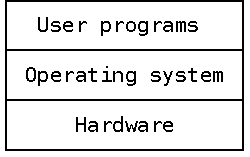
\includegraphics[width=.3\linewidth]{os}
  \caption{操作系统是介于用户进程和硬件之间的软件}
  \label{fig:os}
\end{figure}

现在市面上最流行的操作系统莫过于Windows和Linux。大多数人都是从Windows系
统开始了解计算机和网络的,Windows易用性高,很适合新接触计算机的人上手,
但也因此使多数人对操作系统的选择上产生了很大的误区,认为Windows系统
比Linux系统好用且简单。对于那些使用计算机只是为了上个网看个视频、打打游
戏、查查资料的用户确实使用Windows系统是最简单的。但抛开这些不
谈,Linux是使用命令行字符模式为主要操作方式,而Windows是使用窗口、图标、
鼠标点击形象化的方式为主要操作方式,从这点来看Windows系统就得比Linux系
统要多耗费更多的计算机内存,并且“鼠标+键盘”的操作效率比起使用键盘敲指令
就可以完成操作的效率是要慢很多的。甚至熟练后Linux系统的查资料、看视频等
体验都是要优于Windows系统的。这些只是用户基本体验上的区别,
而Linux与Windows最大的不同在于Linux系统是自由的。自由,不止是说使用这个
系统不出钱,重点是Linux内核是完全开源的,如果本身技术水平比较高的话,甚
至可以用它自己DIY一个只属于自己的任何风格的OS,仔细一想这不是一件非常酷
且很有意思的事吗?而Windows系统的内核是闭源的,所以到现在Linux的版本有
很多很多,而Windows仅仅只有微软公司的Windows XP、Win7、Win11等,用户的
选择很有限。除版本区别外,Linux与Windows还有个很大的区别在于安全性,因
为Linux的软件基本上也都是开源的,在这个大家庭里的很多都是相互扶持的关系,
互帮互助,你需要什么都可以通过一个指令直接获取到软件包直接安装到你的电
脑上。而Windows系统想要个软件,如果不是官方的可能还要担心有没有病毒等,
若是官方的也有可能需要收费购买,破解版又缺乏了安全性并且也是不合法
的\cite{lt2021}。

综上所述,所以我觉得研究并且能够做出一个属于自己的基于Linux技术的OS是
一件很有意义的事,它不但能够令我对Linux的运行逻辑更加清晰,
也能够使我对操作系统开发的了解更加深入透彻。

\section{开发工具及环境}

\subsection{开发工具}

\begin{description}
\item[编辑器:] VIM v0.7.2; Emacs v28.2;
\item[编译器:] GCC v12.2.0;
\item[汇编器:] NASM v2.16.01;
\item[虚拟机:] Bochs v2.6.9\footnote{宿主机如果是Debian GNU/linux可以直
    接敲命令:“sudo apt install vgabios bochs bochs-x bximage”来安
    装bochs。};
\item[Makefile:] GNU Make v4.3.
\end{description}

\subsection{环境配置}

\begin{description}
\item[宿主OS:] Linux v6.1.0-7-amd64 \#1 SMP Debian v6.1.20-2
\item[硬件:] x86\_64
\end{description}

\section{该研究的主要内容}

该研究的主要内容为从操作系统最底层的原理探索一个操作系统从0到1的实现。首先是计算机的
开机过程:引领我们走向计算机这一整个系统的神秘代码,\texttt{0x7C00},一切都要从它开始。计
算机通电开机之后,BIOS便会开始自检,在找到可用的磁盘后,BIOS就会把它的第一个扇区加载到
\texttt{0x7C00},之后由一个512字节的主引导记录MBR\footnote{实际上只有446字节用于引导程序和参数,剩
  下的64字节用于分区表和2字节用于结束标记的\texttt{0x55}和
  \texttt{0xAA}。}从BIOS中接过系统的控制权,也就是CPU的使用权。MBR便是从
\texttt{0x7C00}处接管CPU的,刚好是512字节。之后,MBR寻找操作系统所在的
分区,我们规定用\texttt{0x80}来表示分区上有引导程序,方便MBR从众多分区
中方找到操作系统所在的分区,MBR如果找到了这个分区,就会将CPU使用权交给
这个分区上的引导程序,该引导程序通常就是内核加载器,所以,为了让MBR能
够更方便的在那么大的分区里找到内核加载器,通常我们会把内核加载器的入口
地址固定在分区最开始的扇区,该扇区就是我们熟悉的操作系统引导扇区(MBR
扇区)。而在MBR扇区的前3个字节处存放了跳转指令,目的是为了让MBR找到分
区交接工作后,将处理器带入操作系统引导程序中,至此MBR就完成了所有工作,
CPU的控制权就交到了内核手里。到此为止,计算机也只算是开机了而已,此时计算机的状态就像是在执行代码:
\begin{codeblock}
\begin{ccode}
while(1)
{
  操作系统代码();
}
\end{ccode}  
\end{codeblock}

因此,想让计算机知道我们要让它做什么事就还得需要进程,当然,
一个进程也
只能完成一项工作,在很多时候工作往往并不简单,因此,我们想让进程尽可能的同时多做一些子工作,
而这些“子工作”就是我们熟悉的线程。现在有了进程以及线程,但是计算机仍然在做一个\texttt{while(1)}的循
环,所以还需要给计算机一个中断,让它能够判断出事情的重要程度,也就是优
先级,来选择先把哪件事情
给做好,之后再进行之前没完成的工作,到这才算是实现了一个操作系统\cite{yy2009}。


%%% Local Variables:
%%% mode: latex
%%% TeX-master: "../thesis"
%%% End:
 %%% 论文的目录结构大致如下:
\chapter{系统设计}

“SheepOS”,是我为该操作系统取的一个名字,这名字的由来也很简单,毕竟是自己做的一个OS,那也总得自
己给它取个名字,Sheep其实跟我的名字也有一点关系,在以前初中的时候刚学没几个单词,同学们就
开始取英文名玩儿,他们简单粗暴的给我取了个“Sheep Star”的名字,现在想想还挺好笑的。但
我也并不排斥Sheep这个词,而且我也很喜欢绵羊,所以索性就把我的OS叫做SheepOS了。

\section{总体设计}
\label{sec:overalldesign}

本文主要参照Linux操作系统的内核框架,尝试实现一个带有文件操作功能和命令
行接口的简单操作系统。本系统主要包含以下四个模块:1)启动模块;2)进程
模块;3)数据存储模块;4)外围功能模块。

这四个模块分别有自己负责的范围。其中,启动模块负责从上电开机到操作系统
启动的过程;进程模块负责进程的产生、调度、和管理;数据存储模块实现硬盘、
内存等存储数据的功能,它是后续的文件系统、键盘输入等功能的基础;外围功
能模块建立在前三个模块的基础之上,主要是一些针对文件的操作,包括文件的
打开、关闭、读写、删除等等。这些功能的实现都离不开前三个模块,只有先完
成了前三个模块,才能实现这些基本的功能。

\section{模块设计}

\subsection{启动模块}

启动模块主要涉及BIOS、MBR、Loader、Kernel等部分。在操作系统启动过程中,
先由BIOS来找到MBR,
然后由MBR来引导并加载Loader,再由Loader来加载Kernel。如图
\ref{fig:boot}所示,启动模块的目的可以总结为一个,那就
是加载Kernel。它的详细过程在第\ref{cha:OSboot}章中将会介绍。

\begin{figure}[H]
  \centering
  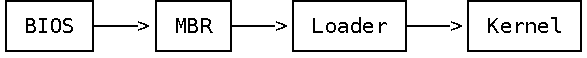
\includegraphics[width=.6\textwidth]{boot}
  \caption{与系统启动相关的各模块}
  \label{fig:boot}
\end{figure}

\subsubsection{计算机的开机过程}

引领我们走向计算机这一整个系统的神秘代
码,\texttt{0x7C00},一切都要从它开始。计算机通电开机之后,BIOS便会开始
自检,在找到可用的磁盘后,BIOS就会把它的第一个扇区加载
到\texttt{0x7C00},之后由一个512字节的主引导记录MBR\footnote{实际上只
  有446字节用于引导程序和参数,剩下的64字节用于分区表和2字节用于结束标
  记的\texttt{0x55}和\texttt{0xAA}。}从BIOS中接过系统的控制权,也就
是CPU的使用权。MBR便是从\texttt{0x7C00}处接管CPU的,刚好是512字节。之
后,MBR寻找操作系统所在的分区,我们规定用\texttt{0x80}来表示分区上有引
导程序,方便MBR从众多分区中方找到操作系统所在的分区,MBR如果找到了这个
分区,就会将CPU使用权交给这个分区上的引导程序,该引导程序通常就是内核加
载器,所以,为了让MBR能够更方便的在那么大的分区里找到内核加载器,通常会
把内核加载器的入口地址固定在分区最开始的扇区,该扇区就是操作系统引导扇
区(MBR扇区)。而在MBR扇区的前3个字节处存放了跳转指令,目的是为了
让MBR找到分区交接工作后,将处理器带入操作系统引导程序中,至此MBR就完成
了所有工作,CPU的控制权就交到了内核手里。到此为止,计算机完成了开机,此
时计算机的状态就像是在执行代码:

\begin{codeblock}
\begin{ccode}
while(1)
{
  操作系统代码();
}
\end{ccode}  
\end{codeblock}


\subsection{进程模块}

进程模块主要包括特权级的转变、用户进程的创建、还有进程调度等方面。有了该模块操作系统才能使用户
程序在一个相对安全的环境中执行,并且能够实现多任务同时进行与切换。在本操作系统中,特权级转
变采用的是中断返回的方法:当中断发生时,在中断入口函数\texttt{intr\%1entry()}中通过\texttt{push}
操作来保存当前任务的上下文数据,因此,之后也需要有相应的\texttt{pop}操作来恢复数据,这属于
\texttt{intr\%1entry()}函数的逆过程,在使用\texttt{pop}操作恢复数据后,CPU就会认为用户进程从中断返回了。
在此操作之后,用户进程将在最低的特权级3下运行,操作系统处于最高特权级0,这样就达到了
该模块的目的。当用户进程处在特权级3之后,进程的创建就是通过一个\texttt{process\_execute()}函数来创建
的,创建成功后再由时钟中断用\texttt{schedule()}从就绪队列中进行调度。详细的步骤在第
\ref{sec:course}节中将会介绍。

\subsection{内存模块}

此模块就是为了进程而存在的,主要为新产生的进程分配对应的内存空间,在进程结束后再对内存进行
回收。内存的创建并不是提前准备好的,它是在需要的时候由程序动态创建的,例如进程需要内存的时
候,会调用相关的函数,然后动态分配并且维护内存块资源,再使用完内存后,还需要把内存回收回去,
而内存的使用情况一直是由位图\footnote{位图是操作系统中常用的一种数据结构,是一个二进制数
  组,其中的每个Bit表示相应的存储快的状态,通常用0表示未使用,1表示已使用。}来进行管理的,
所以无论内存的分配或者释放,本质上其实就是在设置相关位图的相应位,也就是在读写位图。

\subsection{外围功能模块}

在有了启动、进程、内存模块之后,就可以实现一个简单的文件系统,一个简单的shell,shell的一些
简单功能,本文中主要实现的功能有:文件的创建、文件的删除、文件的打开、文件的关闭、文件的写
入、文件的读取、文件的删除这些文件操作。

而在shell中实现了\Ctrl{L}和\Ctrl{U}快捷键,分别是清屏和清除输入,还有一些简单的\texttt{ls}、\texttt{cd}、
\texttt{mkdir}、\texttt{rmdir}操作。 

%%% Local Variables:
%%% mode: latex
%%% TeX-master: "../thesis"
%%% End:
 % thesis/
\chapter{操作系统的启动过程}
\label{cha:OSboot}

\section{基本输入输出系统(BIOS)}
\label{sec:BIOS}

BIOS的全称是Basic Input/Output System,意思就是基本输入输出系统。它是计
算机上第一个运行的软件。当然,它不可能自己加载自己,那么它就只能是由硬
件来加载了,而这个硬件就是CPU\cite{zg2016}。在计算机通电
瞬间,如图\ref{fig:img2-1}所示,寄存器\texttt{CS:IP}会被赋予一个初
值:\texttt{F000:FFF0}。之后,CPU将会执行下面这条指令:
\begin{codeblock}
\begin{nasmcode}
jmp f000:e05b
\end{nasmcode}
\end{codeblock}
\texttt{JMP},顾名思义就是要跳转到内存中的\texttt{F000:E05B}这个地址,
这里就是BIOS待机的地方。\texttt{JMP}到这之后,BIOS被唤醒,得到了软
件接力的第一棒。而BIOS要干的事情就是:
\begin{enumerate}
\item 准备好和基本输入输出相关的函数
\item 检查硬件
\item 将主引导扇区(MBR)的代码加载到内存中的\texttt{0x7C00}位置
\item 跳转到\texttt{0x7C00}
\end{enumerate}

\begin{figure}[H]
  \centering
  \includegraphics[width=.9\linewidth]{图2-1}  
  \caption{Bochs屏幕截图}
  \label{fig:img2-1}
\end{figure}

\section{MBR的工作}
\label{sec:MBR}

MBR,全称是Master Boot Record,主引导扇区,共有512个字节,其结构如图\ref{fig:mbr}所
示。主要由三个部分组成,分别是:
\begin{enumerate}
\item 主引导程序(Bootloader):占扇区前446个字节,在计算机开机,BIOS完成自检后,会将MBR加载
  到内存中,然后执行前446字节的引导程序。
\item 硬盘分区表(DPT):占扇区中间64个字节,主要用来定位各个分区,访问用户数据。
\item MBR结束标志\texttt{0xAA55}:占扇区最后2字节,也被称为魔数。每次执行引导程序时都会检查
  程序的结尾是否是\texttt{0xAA55},若不是的话则会认定这是一个无效的MBR引导扇区,将会中止引
  导。
\end{enumerate}

\begin{figure}
  \centering
  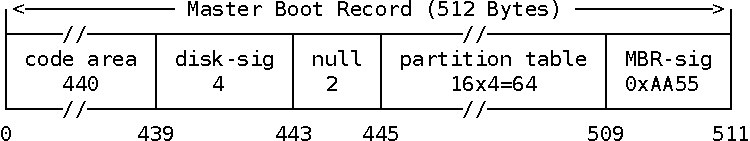
\includegraphics[width=.7\textwidth]{mbr}
  \caption{MBR的结构}
  \label{fig:mbr}
\end{figure}

BIOS在\texttt{0x7C00}处把CPU的控制权交由MBR之后,将会再次进入待机状
态,至此,BIOS的使命就完成了。MBR中的代码部分是由我们自己编写的,它可
以简单到只要如下三条汇编程序语句:%
\begin{enumerate}
\item 告诉汇编器把我们的起始地址编译为\texttt{0x7C00};
\begin{codeblock}
\begin{nasmcode}
 SECTION MBR vstart=0x7c00
\end{nasmcode}
\end{codeblock}
\item \verb'$'表示本行所在的地址,\verb'$-$$'意思是本行到本section的偏移量,MBR必须得填满
  512个字节,而最后两个是固定的\texttt{0x55}和\texttt{0xAA},所以剩下空着的部分用0来填充。
\begin{codeblock}
\begin{nasmcode}
 times 510-($-$$) db 0 
\end{nasmcode}
\end{codeblock}
\item MBR结束;
\begin{codeblock}
\begin{nasmcode}
 db 0x55,0xaa  
\end{nasmcode}
\end{codeblock}  
\end{enumerate}

这样我们就拥有了一个很小的MBR,当然只是这样做的话太不优雅了,屏幕上可能会有很
多乱七八糟的代码,所以还是让我们的MBR不那么简单一点:%

\begin{longlisting}
\begin{nasmcode}
    org 07c00h          ; 告诉编译器程序加载到7c00处
    mov ax, cs          
    mov ds, ax          
    mov es, ax          
    mov ah, 0x6         ; 利用0x60号功能清屏
    mov al, 0x0         ; AL = 上卷的行数(0表示全部)
    mov bx, 0x700
    mov cx, 0x0
    mov dx, 0x184f
    int 10h
    call DispStr        ; 调用显示字符串例程
    jmp $               ; 无限循环
DispStr:
    mov ax, BootMessage
    mov bp, ax          ; ES:BP = 串地址
    mov cx, 16          ; CX = 串长度
    mov ax, 01301h      ; AH = 13,  AL = 01h
    mov bx, 000ch       ; 页号为0(BH = 0) 黑底红字(BL = 0Ch,高亮)
    mov dl, 0
    int 10h             ; 10h 号中断
    ret
BootMessage:        db  "Hello, OS world!"

times   510-($-$$)  db  0   ; 填充剩下的空间,使生成的二进制代码恰好为512字节
dw  0xaa55                  ; 结束标志
\end{nasmcode}
\end{longlisting}

如图\ref{fig:img2-2}所示,一个最小的操作系统就完成了。

\begin{figure}[H]
  \centering
  \includegraphics[width=.7\linewidth]{图2-2}
  \caption{Hello, OS World!}
  \label{fig:img2-2}
\end{figure}

整个界面没有显示其它的参数信息,仅有刚刚代码中打印出的\emph{Hello, OS World!}字
样,这小小的512个字节,如果按代码量来算的话甚至没有512字节,但它已经坐
在了操作系统的位置上,接下来的工作都将建立在该基础之上,一步一步的来完
善我的SheepOS\footnote{我自己给它取的一个名字,因为我很喜欢绵羊所以就把
  我的OS叫做SheepOS了。}。至此,MBR已经从BIOS上接管了CPU的使用权,下面就该
轮到Loader出场了。

\section{Loader的工作}
\label{sec:Loader}

MBR在完成跟BIOS的交接后,需要解决三个问题:1)从硬盘上找
到Loader;2)把Loader搬运到内存中的什么地方;3)怎样搬运。其中第1、2条
其实是由自己定义的,可以自己选择把Loader放在硬盘里的任何一个地址,我选
择放在了第二扇区,所以就需要MBR去硬盘的第二扇区寻找Loader。那么找到Loader后
要搬运到哪呢?

\begin{figure}
  \centering
  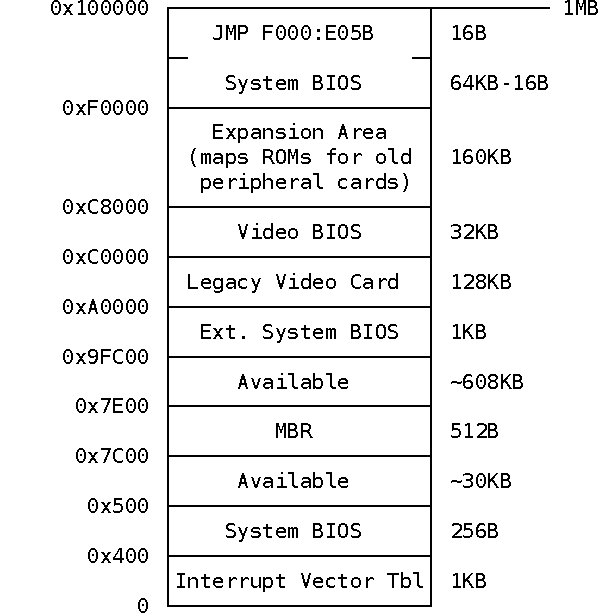
\includegraphics[width=.4\linewidth]{boot-mem}
  \caption{实模式下的内存布局}
  \label{fig:neicun}
\end{figure}

如图\ref{fig:neicun}所示,有两个可用的区
域\texttt{0x7E00~0x9FBFF}和\texttt{0x500~0x7BFF},我选择把它放
在\texttt{0x900}这个地方,所以最终MBR就会把Loader搬运到\texttt{0x900}这
个地方。

\section{内核的启动}
\label{sec:kernel}

\subsection{从实模式到保护模式}
\label{subsec:protect}

在Loader被搬运到\texttt{0x900}之后,需要将操作系统由实模式转变到保护模式\cite{LWY2013},原因在于:
\begin{enumerate}
\item 实模式下操作系统和用户程序会属于同一个特权级。
\item 逻辑地址 = 物理地址,顾名思义就是用户程序引用的地址最终都指向真实的物理地址。
\item 用户程序能够自由地修改段基址。
\item 当需要访问超过64KB内存的区域时,要切换段基址。
\item 浪费计算机资源,因为一次只能够运行一个程序。
\item 一共只有20条地址线,加起来最大的可用内存也仅有1MB。
\end{enumerate}

所以需要将操作系统引导到保护模式下才可以既安全,又能充分地利用计算机的
资源,还不用过于担心内存问题。因为实模式的寻址方式是“(段基址:段内偏移
地址)”的形式;而保护模式的寻址方式是“(选择子:段:偏移地址)”,所以保护
模式还需要段描述符来描述一个段的信息,一个段描述符是8个字节,多个段描述
符就构成了段描述符表也就是“GDT”\footnote{GDT(Global Descriptor Table)\cite{chxs2012},全局描述符表,一个
  CPU对应一个GDT,它可以被放在内存的任何地方,也就是说它是全局的,存放在内存中的某个位置,
  而这个位置将由我们来指定}。因此第一步就是打开A20地址线(详见第\ref{sec:inprotect}节),让操作系
统能够访问更大的空间,方法也很简单,就是把\texttt{0x92}的第一个比特
置1就可以了。代码如下:
\begin{codeblock}
\begin{nasmcode}
in al, 0x92
or al, 0000_0010B
out 0x92, al
\end{nasmcode}  
\end{codeblock}
仅需要3行代码,就可以打开A20地址线。
之后加载之前写好的GDT。
最后一步就是将保护模式的开关 --- \texttt{CR0}寄存器 --- 的\texttt{PE}比特置1,也很简单,就三行代码:

\begin{codeblock}
\begin{nasmcode}
mov eax, cr0
or  eax, 0x00000001
mov cr0, eax
\end{nasmcode}  
\end{codeblock}

至此,操作系统已经成功进入了保护模式,接下来就是本节的主角“内核”登场了。

\subsection{内核初始化}

Loader把内核从硬盘上读出来,然后加载到内存中去,至此,软件接力棒就交到
了最后一位选手 --- 内核 --- 手里,这就是操作系统从电脑开机到接
管CPU使用权的一个大致过程。内核的代码如下:

\begin{codeblock}
\begin{ccode}
int main(void)
{
    while(1);
}
\end{ccode}  
\end{codeblock}

没错,就可以是这么一个简单的程序,操作系统实质上从头到尾也就是在做这么一件
简单的事情。


%%% Local Variables:
%%% mode: latex
%%% TeX-master: "../thesis"
%%% End:
 %       ├── doc/
\chapter{SheepOS的实现}

上一章提到过“SheepOS”,这名字的由来也很简单,毕竟是自己做的一个OS,那也总得自
己给它取个名字,Sheep其实跟我的名字也有一点关系,在以前初中的时候刚学没几个单词,同学们就
开始取英文名玩儿,他们简单粗暴的给我取了个“Sheep Star”的名字,现在想想还挺好笑的。但
我也并不排斥Sheep这个词,而且我也很喜欢绵羊,所以索性就把我的OS叫做SheepOS吧。

\section{系统启动过程}
\label{sec:booting}

当按下计算机的开机键后,计算机开始自检,之后运行第一个软
件BIOS。BIOS的工作在第\ref{sec:BIOS}节有过介绍,在此就不再赘述了。
在BIOS把CPU使用权交给了MBR之后,MBR会在硬盘上的第二个扇区找到我们
的\texttt{Loader.bin}并把它加载到内存中去,之后操作系统将在Loader中跳入
保护模式,并且由Loader来加载内核。

\subsection{读取硬盘扇区}

为了让MBR能够定位Loader,我们需要一个\texttt{rd\_disk()}函数来读
取Loader所在硬盘的扇区。该函数的完整代码在附录\ref{fsec:loader_disk}中。该函
数的工作步骤大致如下:
\begin{enumerate}
\item 备份\texttt{eax}和\texttt{cx}寄存器;
\item 设置要读取的扇区数;
\item 将LBA\footnote{Logical Block Address, 逻辑块地址,可以理解为硬盘的物理地址}
地址存入\texttt{0x1F3~0x1F6};
\item 向\texttt{0x1F7}端口写入读命令,\texttt{0x20};
\item 检测硬盘状态;
\item 从\texttt{0x1F0}端口读数据;
\end{enumerate}

之前在第\ref{sec:Loader}节中提到过,我选择将我的Loader放在硬盘的第二个
扇区,所以,在MBR中我会:
\begin{codeblock}
  \begin{nasmcode}
    mov al,2
  \end{nasmcode}
\end{codeblock}
来让MBR来读取硬盘的第二个扇区,在这儿就可以找到
\texttt{Loader.bin},这些就是MBR对硬盘的操作了。
在MBR找到Loader之后会把它搬运到之前写好的位置:\texttt{0x900}处,然后就会把CPU的使用权交给
Loader, MBR的工作至此也就结束了。

\subsection{进入保护模式}
\label{sec:inprotect}

保护模式的必要性在之前第\ref{subsec:protect}节中已经提及,并且大
致介绍了进入保护模式的方法。保护模式是在\texttt{Loader.bin}中进入的。在
上一节中,MBR已经完成了它的工作,将Loader引导到了合适的位置,并把CPU的使用权交
给了Loader。此时的\texttt{Loader.bin}其实已经超过了512个字节,所以
在MBR中加载Loader的读入扇区数要扩大,为了避免后续频繁更改,索性就把它改
成读入第4扇区。\par\bigskip

\begin{itemize}
\item[] 
  \begin{nasmcode}
    mov cx,4
    call rd_disk
  \end{nasmcode}

\item 描述Loader的起始地址:
\begin{nasmcode}
  LOADER_BASE_ADDR equ 0x900   ;equ是nasm的提供的伪指令,意为equal,
                               ;用于给表达式起个意义更明确的符号名
\end{nasmcode}

\item 配置全局描述符表GDT(GDT的概念详见第\ref{subsec:protect}节);
\begin{nasmcode}
DESC_G_4K   equ   1_00000000000000000000000b   
DESC_D_32   equ    1_0000000000000000000000b
DESC_L      equ     0_000000000000000000000b    ;64位代码标记,此处标记为0便可。
DESC_AVL    equ      0_00000000000000000000b    ;cpu不用此位,暂置为0  
DESC_LIMIT_CODE2  equ 1111_0000000000000000b
DESC_LIMIT_DATA2  equ DESC_LIMIT_CODE2
DESC_LIMIT_VIDEO2 equ  0000_000000000000000b
DESC_P            equ     1_000000000000000b
DESC_DPL_0        equ      00_0000000000000b
DESC_DPL_1        equ      01_0000000000000b
DESC_DPL_2        equ      10_0000000000000b
DESC_DPL_3        equ      11_0000000000000b
DESC_S_CODE       equ        1_000000000000b
DESC_S_DATA       equ DESC_S_CODE
DESC_S_sys        equ        0_000000000000b

DESC_TYPE_CODE    equ  1000_00000000b   ;x=1,c=0,r=0,a=0
                                        ;代码段是可执行的,非依从的,不可读的,已访问位a清0.  
                               
DESC_TYPE_DATA    equ  0010_00000000b   ;x=0,e=0,w=1,a=0
                                        ;数据段是不可执行的,向上扩展的,可写的,已访问位a清0.

DESC_CODE_HIGH4 equ (0x00 << 24) + DESC_G_4K + DESC_D_32 + DESC_L + DESC_AVL + DESC_LIMIT_CODE2 + DESC_P + DESC_DPL_0 + DESC_S_CODE + DESC_TYPE_CODE + 0x00

DESC_DATA_HIGH4 equ (0x00 << 24) + DESC_G_4K + DESC_D_32 + DESC_L + DESC_AVL + DESC_LIMIT_DATA2 + DESC_P + DESC_DPL_0 + DESC_S_DATA + DESC_TYPE_DATA + 0x00

DESC_VIDEO_HIGH4 equ (0x00 << 24) + DESC_G_4K + DESC_D_32 + DESC_L + DESC_AVL + DESC_LIMIT_VIDEO2 + DESC_P + DESC_DPL_0 + DESC_S_DATA + DESC_TYPE_DATA + 0x0b
\end{nasmcode}
\end{itemize}

\begin{figure}
  \centering
  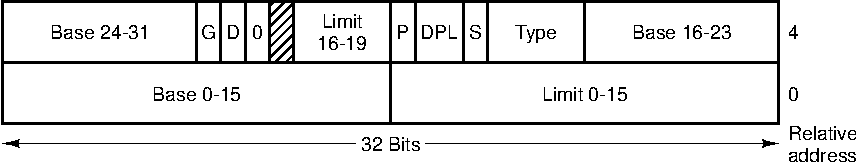
\includegraphics[width=.7\linewidth]{gdt}
  \caption{段描述符格式}
  \label{fig:gdt}
\end{figure}

图\ref{fig:gdt}所示为GDT的标准格式,我们的GDT表就是根据该格式来进行配置
的。值得注意的是从\texttt{DESC\_DPL\_0}到\texttt{DESC\_DPL\_3}这四行代
码,他们代表的是保护模式特有的特权级概念。如图\ref{fig:tequan}所示,特
权级号越小权限越大,因此在进入保护模式后,操作系统的特权级应当是在0处,
而用户程序位于最低的特权级3处;若是实模式的话所有的一切都存在于同一个特
权级,这样实在是太危险了,所以这就是要费尽千辛万苦也要使操作系统进入保
护模式的原因。

\begin{figure}[H]
  \centering
  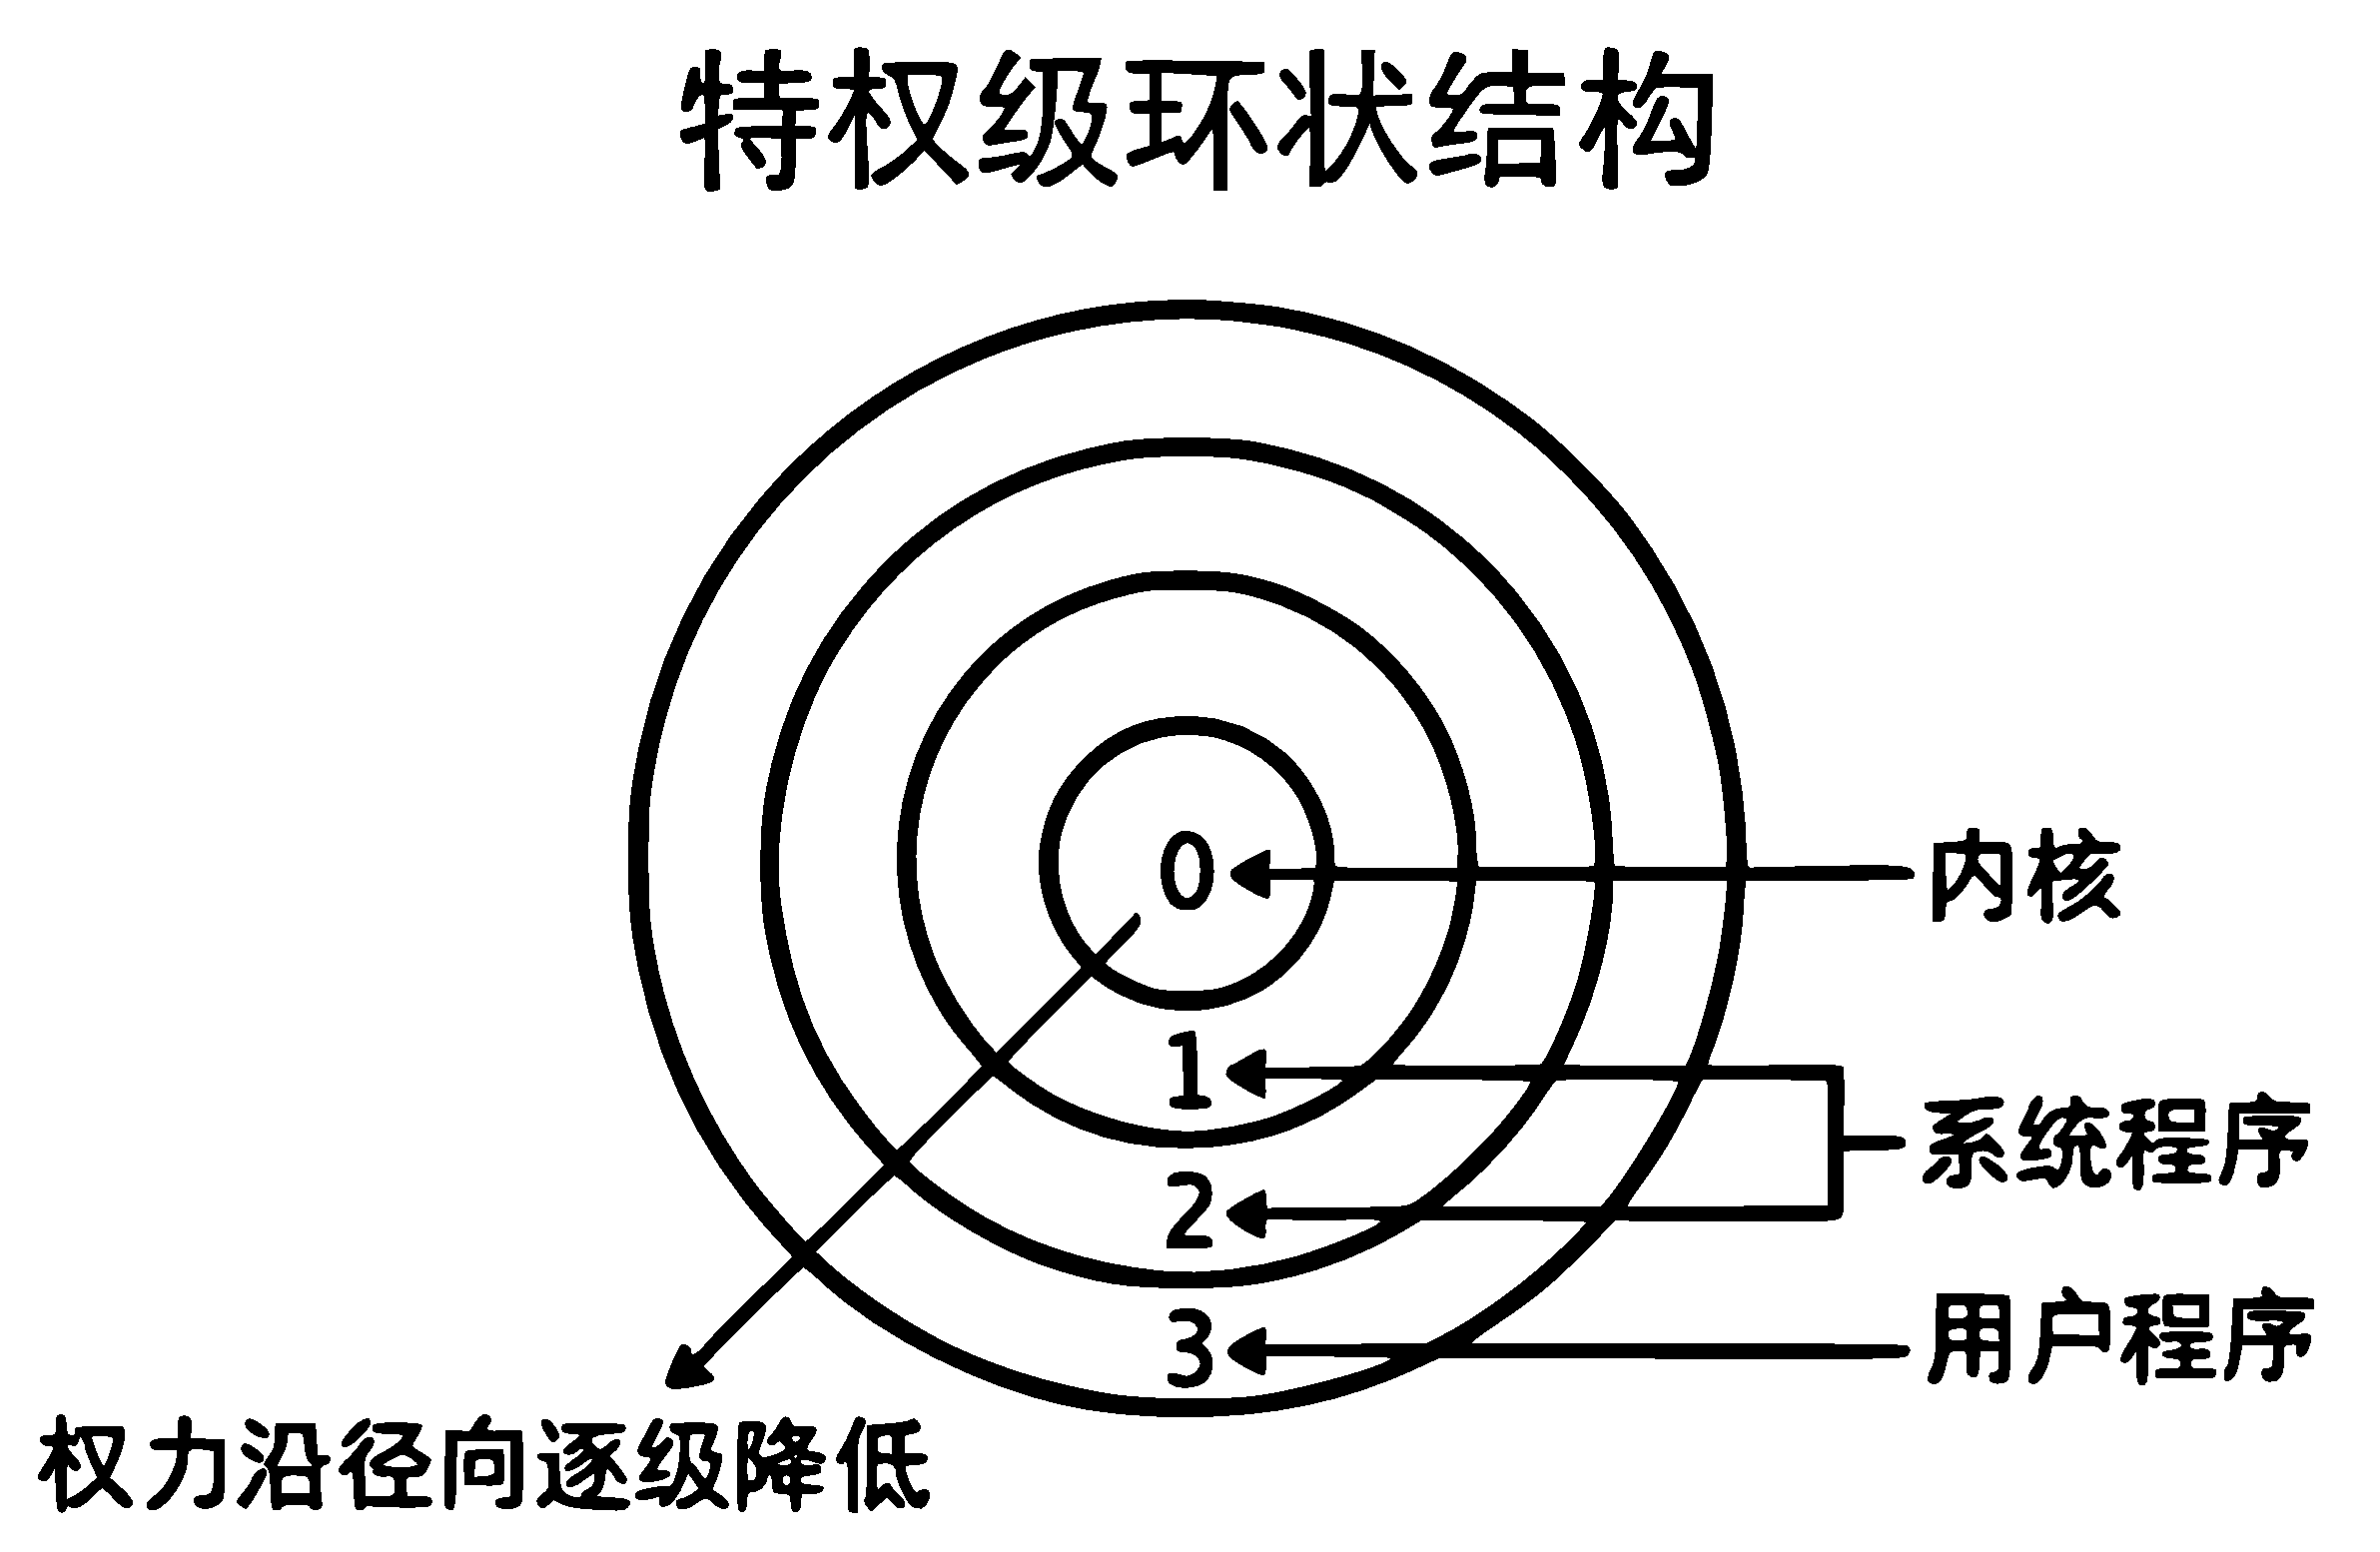
\includegraphics[width=.4\linewidth]{priv}
  \caption{特权级结构}
  \label{fig:tequan}
\end{figure}

关于A20地址线打开与否的区别:
\begin{itemize}
\item 如果A20地址线被打开,当访问到\texttt{0x100000~0x10FFEF}之间的地址时,CPU将真正访问到这块物理
  地址。
\item 如果A20地址线未被打开,当访问\texttt{0x100000~0x10FFEF}之间的地
  址时,CPU将采用8086/8088的地址回绕。实模式下的地址线是20位,最大寻址
  空间是1MB,即\texttt{0x00000~0xFFFFF}。超出1MB内存的部分在逻辑上虽然
  也是正常的,但物理内存中没有与之对应的部分,所以为了让“(段:偏移地
  址)”的策略可用,CPU会采取将超过1MB的部分自动绕回0地址的做法,继续
  从0地址开始映射,这就叫做地址回绕。如:\texttt{0x100000},由于没有第21位地址线,
  相当于丢掉了进位1,将会变成\texttt{0x00000}。
\end{itemize}

所以,我们进入保护模式就需要抛弃地址回绕这种做法,相应的也就需要超过20条地址去访问更大的空间,
而打开A20地址线就是以此为目的,打开的方法在\ref{subsec:protect}的时候也已经介绍过,在此就
不过多赘述了。最后,
\begin{codeblock}
  \begin{nasmcode}
    jmp dword SelectorCode32:0
  \end{nasmcode}
\end{codeblock}
将\texttt{CR0}寄存器的PE比特置1后,我们的操作系统就成功的跳入了保护模式!

\subsection{加载内核}
\label{subsec:kernel}

在加载Kernel之前,得先获取物理内存容量,只有掌握了物理内存的大小,才能
更好地操作虚拟内存。在此,我们利用BIOS中断号\texttt{0x15}的子功能来获
取物理内存的大小。代码详见附录\ref{fsec:loader_15h}。其工作过程大致如下:
\begin{enumerate}
\item 定义好调用之前输出的寄存器\texttt{ECX}和\texttt{EDX};
\item 调用int \texttt{0x15}号中断;
\item 在返回后输出的CF位为0时,寄存器\texttt{EAX}、\texttt{ES:DI}、\texttt{ECX}、
  \texttt{EBX}便会出现对应的结果。
\end{enumerate}

如图\ref{fig:xp}所示,在执行\texttt{xp 0xB00}后,结果是\texttt{0x02000000},换算成十进制正好是32MB,故检测结果是正
确的。到这儿我的SheepOS已经有了物理内存检测的功能,这下就能够对物理内存做到心中有数了。
虽然对物理内存的多少已经能够掌握了,但这些内存对于以后整个计算机而言还是太小了,在保护模式
中,地址空间达到了4GB,但目前是所有的进程包括操作系统共享这一个4GB,这样听起来是不是就觉得
4GB其实也很小,所以就需要对内存进行分页。

\begin{figure}
  \centering
  \includegraphics[width=15cm]{图3-3}
  \caption{用xp命令查看物理内存}
  \label{fig:xp}
\end{figure}

图\ref{fig:fenye}所示是分页机制的工作原理,在打开分页机制后,原本的保护
模式的寻址方式又将改变了,将变成“(GDT:虚拟地址:页:物理地址)”这样一个
寻址方式。因为有了分页机制后,就可以将线性地址转换成物理地址,且可以用
大小相等的页来代替大小不等的段,具体如图\ref{fig:fenyezy}所示。

\begin{figure}
  \centering
  \includegraphics[width=12cm]{图3-5}
  \caption{分页机制}
  \label{fig:fenye}
\end{figure}

\begin{figure}[H]
  \centering
  \includegraphics[width=12cm]{图3-4}
  \caption{分页机制的作用}
  \label{fig:fenyezy}
\end{figure}

虚拟地址与物理地址之间有一个映射关系,它们之间的转换是以页(4KB)为单位的。
一个页表有1024个页表项,一个页表项指向一个页的首地址,那我们的4GB就需要1M个页,而一个页是
4KB,所以就需要1024个页表,也就是一个页表目录(二级页表)。而启用分页机制需要按顺序做3件事:
1)准备好页表目录和页表;2)将页表地址写入控制寄存器\texttt{CR3};3)寄存器CR0的PG比特置1。
页表目录和页表的创建过程大致如下:

\begin{enumerate}
\item 需要先把页目录占用的空间逐字节清0;
\item 之后创建页目录项(PDE);
\item 再将页目录项0和0xc00都存为第一个页表的地址;
\item 创建页表项(PTE);
\item 创建内核其它页表的PDE;
\item 把页表地址写入CR3;
\item 将CR0的PG位置1;
\item 最后在开启分页后,用GDT新的地址重新加载;
\end{enumerate}
代码详见附录\ref{fsec:loader_page}。

如图\ref{fig:infogdt},GDT的段基址已经变成了\texttt{0xc0000900},段描述符的段基址也变成\texttt{0xC00B8000},而
不是\texttt{0xB8000}了,说明我们的SheepOS已经成功进入了分页机制的运行模式。
\begin{figure}[H]
  \centering
  \includegraphics[width=15cm]{图3-6}
  \caption{分页后GDT的变化}
  \label{fig:infogdt}
\end{figure}

接下来就该加载我们SheepOS的“心脏” --- 内核\cite{RL2011}了,加载内核到内存这一步跟MBR的工作基本上都是同样的,首先第一步就是像把\texttt{Loader.bin}放到第2扇区
那样把\texttt{Kernel.bin}放到自己想放的位置上去,因为Loader在第2扇区上,第0扇区放的是MBR,如果放在第
1扇区的话感觉太过拥挤,并且最好给Loader多预留些位置,所以我选择把\texttt{Kernel.bin}放到第7扇区,确
定好要放的扇区的位置后,就得用dd命令往磁盘上写了:

\begin{shellcode}
dd if=kernel.bin of=/SheepOS/hd60M.img bs=512 count=200 seek=7 conv=notrunc  
\end{shellcode}

\begin{itemize}
\item \texttt{seek}为7,目的是越过前7个扇区(第0 \char`~{} 6个扇区),
  我们在第7个扇区写入内核。
\item \texttt{count}为200,目的是一次往参数\texttt{of}指定的文件中写
  入200个扇区。
\end{itemize}

这样,\texttt{Kernel.bin}就被成功的写入磁盘了,接下来就该让Loader去找
到Kernel然后把它从硬盘上搬运到内存中去,跟之前MBR搬运Loader一样,我们还
需要一个缓冲区,如图\ref{fig:hc}所示,跟之前Loader一样,有两个可用区域,
准确的说应该是三个,因为现在MBR也结束任务了,所以之前MBR所占用的区域现
在也能够使用了。

\begin{figure}[H]
  \centering
  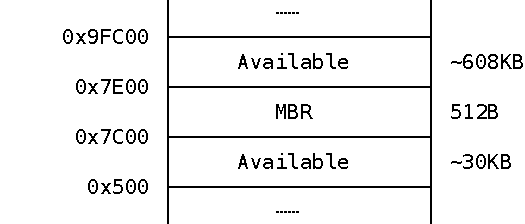
\includegraphics[width=.4\linewidth]{boot-mem2}
  \caption{可用缓冲区}
  \label{fig:hc}
\end{figure}

将来内核文件肯定会越来越大,所以,为了能够预留出足够的空间,我会
把\texttt{Kernel.bin}加载到地址较高的空间,但内核映像要放置在较低的地址
中,因为\texttt{Kernel.bin}在被Loader加载之后就没用了,之后,内核映像在
向高地址处扩展的时候也可以覆盖之前加载到高地址的\texttt{Kernel.bin}所占
用的空间。所以我决定把Kernel加载到\texttt{0x70000}这个地址,当然这个地
址可以随意取,只要取的空间不要比内核还小就行\cite{DM2006}。Loader加载Kernel到内存的
代码也很简单,如下:

\begin{nasmcode}
   KERNEL_START_SECTOR equ 0x200
   KERNEL_BIN_BASE_ADDR equ 0x70000
   mov eax, KERNEL_START_SECTOR        ; kernel.bin所在的扇区号
   mov ebx, KERNEL_BIN_BASE_ADDR       ; 从磁盘读出后,写入到ebx指定的地址
   mov ecx, 200                ; 读入的扇区数

   call rd_disk_32
\end{nasmcode}

其中,\texttt{0x200}是我们为\texttt{Kernel.bin}设置的地址,\texttt{0x70000}是Loader在\texttt{0x200}找到\texttt{Kernel.bin}后加载到的地址。
在Loader把Kernel加载到\texttt{0x70000}之后,还需要对内核进行一下初始化
(程序代码参见附录\ref{fsec:kernel_init}),其过程大致如下:
\begin{enumerate}
\item 将\texttt{kernel.bin}中的段拷贝到各个段自己被编译的虚拟地址处;
\item 把这些段单独提取到内存中;
\item 判断段类型,如果不是\texttt{PT\_NULL},就把这些段拷贝到编译的地址中。
\end{enumerate}
至此,我们的SheepOS已经成功拥有内核了,且之后CPU的控制权也将交给内核。

\section{简单的屏幕输出}

在之前没有我们自己的\texttt{Print}函数,想在屏幕上输出文本时,不是利用BIOS中断就是利用系统调用,太
不方便,所以该节将会为我的SheepOS增加属于它自己的\texttt{Print}函数。要实现一个\texttt{Print}函数大致可以
分为以下几个步骤(具体代码参见\ref{fsec:put_char}):

\begin{enumerate}
\item 备份寄存器;
\item 获取光标当前所处的位置坐标,该位置就是下一个可打印字符的位置;
\item 获取需要打印的字符;
\item 判断字符类型;如回车、换行、退格则会被特殊处理,除此之外将会直接输出显示;
\item 判断需不需要滚屏;
\item 更新光标的位置坐标,让它指向下一个打印字符的位置;
\item 恢复寄存器。
\end{enumerate}
这样就实现了对单个字符的打印,效果如图\ref{fig:print_char}所示,这里只实现了对单个字符的
print,目前该效果是由多个\texttt{put\_char}来打印字符拼到一起来实现的

\begin{figure}[H]
  \centering
  \includegraphics[width=12cm]{图3-8}
  \caption{字符打印}
  \label{fig:print_char}
\end{figure}

\begin{codeblock}
\begin{ccode}
int main(void)
{
    put_char('k');
    put_char('e');
    put_char('r');
    put_char('n');
    put_char('e');
    put_char('l');
    put_char('\n');
    put_char('1');
    put_char('2');
    put_char('\b');
    put_char('3');
    while(1);
}
\end{ccode}
\end{codeblock}

这样就形成了图\ref{fig:print_char}中的效果,在字符“kernel”最后换行符\verb|"\n"|起到了效果,
成功换了行,而最后的“1”和“3”便是2和3之间的退格键将字符“2”删除了,只留下了“1”和“3”。

\subsection{字符串的打印}
\label{subsec:str}

单个字符的打印我们已经实现了,而对于字符串Str的打印其实就是对单个字符打印函数进行一个封装。
代码如下:

\begin{nasmcode}
global put_str
put_str:
;由于本函数中只用到了ebx和ecx,只备份这两个寄存器
   push ebx
   push ecx
   xor ecx, ecx		      ; 准备用ecx存储参数,清空
   mov ebx, [esp + 12]	      ; 从栈中得到待打印的字符串地址 
.goon:
   mov cl, [ebx]
   cmp cl, 0		      ; 如果处理到了字符串尾,跳到结束处返回
   jz .str_over
   push ecx		      ; 为put_char函数传递参数
   call put_char
   add esp, 4		      ; 回收参数所占的栈空间
   inc ebx		      ; 使ebx指向下一个字符
   jmp .goon
.str_over:
   pop ecx
   pop ebx
   ret
\end{nasmcode}

在有了\texttt{put\_char}之后\texttt{put\_str}就没那么复杂了,无非就是多调用几个\texttt{put\_char}来进行打印最终达到字
符串的效果,只不过封装以后打印字符串就不用像之前那么繁琐,使用很多行代码来实现。效果如图\ref{fig:print_str}:

\begin{figure}[H]
  \centering
  \includegraphics[width=12cm]{图3-9}
  \caption{打印字符串}
  \label{fig:print_str}
\end{figure}

第一次做到这的时候心里其实是很激动的,因为自己的操作系统第一次在上面打印出来自己的名字和学号以
及想要打印的东西。在有了\texttt{put\_str}之后打印这些字符就变得容易了许多:

\begin{codeblock}
\begin{ccode}
void main(void)
{
   put_str("I am str!\n");
   put_str("20211159013 CynYang\n");
   put_str("this is my OS!\n");
   while(1);
}
\end{ccode}  
\end{codeblock}

像这么多个字符也只需要三行代码,如若不是为了美观加上换行符的效果的话其实一行也就够了。

\subsection{整数的打印}
\label{subsec:int}
既然SheepOS有了能够打印Str的功能,那怎么能没有数字打印呢,要求也不高,就先让它能够打印整数
数字就足够了,原理就是将数字9转变为字符的'9'来输出,提到这个转换当然就不难想到ASCII码了,
在ASCII码表中,字符‘0’~‘9’的范围是48~57,大写字母‘A’~‘Z’的范围是65~90,所以
\begin{itemize}
\item 对数字的处理就是:0~9之间的数字,用该数字加上字符'0'的ASCII码48;
\item 对字母的处理就是:A~F之间的数字,用该数字减去10后再加上字符'A'的ASCII码65;
\end{itemize}
代码详见附录\ref{fsec:put_int}
现在SheepOS已经有了能够打印整形Int的功能了。

\begin{ccode}
void main(void)
{
   put_str("I am Str\n");
   put_str("20211159013 CynYang\n");
   put_int(0);
   put_char('\n');
   put_int(9);
   put_char('\n');
   put_int(0x00021a3f);
   put_char('\n');
   put_int(0x12345678);
   put_char('\n');
   put_int(2023-04-03);
   while(1);
}
\end{ccode}

\begin{figure}[H]
  \centering
  \includegraphics[width=12cm]{图3-10}
  \caption{打印整形字符int}
  \label{fig:print_int}
\end{figure}
看看效果如何,如图\ref{fig:print_int}所示。
它将我们输入的数字经过ASCII码表转换成对应的字符成功输出了!现在SheepOS已经拥有了打印\texttt{Char}、
\texttt{Str}、\texttt{Int}三种类型字符的能力,这将为后面的工作提供很多便利。

\section{中断}
\label{sec:interrupt}

我们知道现在操作系统一直在做一件事情,那就是
\begin{codeblock}
\begin{ccode}
while(1)
{
  操作系统代码();
}
\end{ccode}  
\end{codeblock}
不论我们在其中完成了但是功能,他都是在进行一个死循环,要是没有中断的话,我们也许都不能一边
处理图片,一边敲键盘聊天。就好似你正在玩一个游戏,但现在得跟朋友出去吃饭或是门铃响了要去开
门,若是没有暂停功能的话我们应该很难马上放开这个游戏去做别的事吧。操作系统的中断亦是如此,
正是因为有了中断,我们才能够同时享受计算机的多种服务。中断又分为两种:
\begin{itemize}
\item 外部中断:外部中断顾名思义就是CPU外部的中断,所以又叫做硬件中断。这个中断信号都是来自外部硬件的,如
网卡、磁盘控制器、键盘、鼠标、音频等等,与内部中断不同,它是异步的,就算有正在运行的指令,
它也能够发生。
\item 内部中断:又称为软中断,它通常作为CPU的异常处理,中断存在的意义主要是为了让计算机能够
  实现多任务,包括用户程序之间的切换、软件与软件之间的并存都需要有中断才能实现。
\end{itemize}

\subsection{中断描述符表}

中断描述符表就是保护模式下用于存储中断处理程序入口的表,当CPU收到一个中
断后,需要用中断向量在此表中检索对应的描述符,然后在描述符中找到中断处
理程序的起始地址,之后执行中断处理程序。如表\ref{tbl:idt}所示
\footnote{来源:\url{https://en.wikipedia.org/wiki/Interrupt_descriptor_table}},第一
列\texttt{INT\_NUM}表示中断向量号,共有255个,中断的机制就是在收到一个
中断信号后,调用相对应的中断处理程序,所以CPU在收到中断信号后,会根据中
断向量号去到中断描述符表中找到相应的中断程序的地址。

\begin{table}[!ht]
  \centering  \caption{中断描述符表\label{tbl:idt}}
  \begin{tblr}{width=\textwidth,colspec={rX[l]},hline{1,2,Z}}
INT\_NUM&Short Description\\
0x00   &Division by zero\\
0x01   &Single-step interrupt\\
0x02   &NMI\\
0x03   &Breakpoint\\
0x04   &Overflow\\
0x05   &Bound Range Exceeded\\
0x06   &Invalid Opcode\\
0x07   &Coprocessor not available\\
0x08   &Double Fault\\
0x09   &Coprocessor Segment Overrun\\
0x0A   &Invalid Task State Segment\\
0x0B   &Segment not present\\
0x0C   &Stack Segment Fault\\
0x0D   &General Protection Fault\\
0x0E   &Page Fault\\
0x0F   &reserved\\
0x10   &x87 Floating Point Exception\\
0x11   &Alignment Check\\
0x12   &Machine Check\\
0x13   &SIMD Floating-Point Exception\\
0x14   &Virtualization Exception\\
0x15   &Control Protection Exception\\
  \end{tblr}
\end{table}
% \begin{figure}[H]
%   \centering
%   \includegraphics[width=12cm]{图3-11}
%   \caption{中断向量表}
%   \label{fig:zdxl}
% \end{figure}

\subsection{中断控制器8259A}

认识中断的概念后,我们发现我们的操作系统真是太忙了,计算机上若是插入一个鼠标,操作系统要加
载一下,插入一个键盘,操作系统也要加载一下,本来操作系统就有很多自己的事情需要做了,所以就
需要一个部件来对这些中断进行统一的管理,而这个部件就是可编程中断控制器\texttt{8259A}。
\texttt{8259A}的作用是负责所有来自外设的中断,且它是可编程的,应该可以把它称为是打开中断的入口了。
计算机内有两片\texttt{8259A}芯片,被称为主片和从片,如图\ref{fig:8259A}。

\begin{figure}[H]
  \centering
  \includegraphics[width=12cm]{图3-13}
  \caption{8259A芯片}
  \label{fig:8259A}
\end{figure}

\texttt{8259A}的芯片是直接安装在主板上的,所以可以直接对其进行操作,例如我们移动了一下鼠标,如图
\ref{fig:8259A}在\texttt{8259A}的从片\texttt{IRQ12}引脚处就会收到一个高电频,之后从片就会把该信息通过\texttt{8259A}主
片的\texttt{IRQ2}引脚传递到主片上,再从主片直接反映到CPU上说鼠标将要移动了请求CPU来处理。
那么处理其他中断也是一样的,在\texttt{8259A}收到一个优先级为多少的
中断后会告诉CPU:这是优先级靠前或是靠后的中断,需要进行处理。如图\ref{fig:interrupt_a}
在CPU收到后会根据中断向量号在中断描述符表中进行索引然后找出相应的选择子和偏移地址,在得到
选择子与偏移地址后,再到GDT中去寻找对应的描述段,之后就再在内存中找到该描述段的代码然后再
去执行。
进入中断的方法就是Kernel上调用中断处理函数,代码详见\ref{app:int_a}和\ref{app:int_b},
其过程如下:

\begin{enumerate}
\item 如果是从片上进入的中断,除了往从片上发送\texttt{EOI}外,还要往主片上发送\texttt{EOI};
\item 调用\texttt{idt\_table}中的C版本中断处理函数;
\item 存储各个中断入口程序的地址,形成\texttt{intr\_entry\_table}数组
\end{enumerate}

\begin{figure}[H]
  \centering
  \includegraphics[width=12cm]{图3-12}
  \caption{中断过程}
  \label{fig:interrupt_a}
\end{figure}

如上图\ref{fig:8259A},当向主片\texttt{0xA0}地址和从片\texttt{0x20}地址发送\texttt{EOI}后,就代表告诉\texttt{8259A}中断程序处理
结束了。

在进入中断前,还需要先保存中断发生前上下文的环境,以免发生数据丢失的情况,这里使用\texttt{PUSHAD}指
令压栈压入32位寄存器:
\begin{codeblock}
\begin{nasmcode}
   push ds
   push es
   push fs
   push gs
   pushad
\end{nasmcode}  
\end{codeblock}

在中断调用完后也需要用\texttt{POPAD}来恢复之前的环境:
\begin{codeblock}
\begin{nasmcode}
add esp, 4    ; 跳过中断号
   popad
   pop gs
   pop fs
   pop es
   pop ds
   add esp, 4 ; 跳过error_code
   iretd
\end{nasmcode}  
\end{codeblock}

至此就是\texttt{8259A}控制器的相关中断内容。

\subsection{键盘输入}

我们的SheepOS现在已经有了中断,而在之前的图\ref{fig:8259A}上不难发现\texttt{8259A}主片\texttt{IRQ1}引脚对应
的是键盘,所以可以大胆试想一下,是不是我们的SheepOS即将可以用键盘直接在屏幕上进行输入了?
答案是肯定的。

在此之前,首先得了解下键盘敲击的过程。在我们的键盘中有着一个名为“键盘编译器”的芯片,它通常
是\texttt{8048}以及兼容芯片,作用就是监控键盘的输入,然后把数据发送给计算机,当然计算机主板上也有一
个键盘控制器,专门接受和解码来自键盘的数据,然后跟\texttt{8259A}和各个软件之间进行通信。敲击键盘的
步骤可以分为三种情况:
\begin{enumerate}
\item 按下
\item 保持按下的状态
\item 松开
\end{enumerate}
键盘按下松开后产生的编码叫做“扫描码”,当键盘按下和保持按下的时候产生\texttt{Make Code},而当松开
后会产生\texttt{Break Code}。在知道有扫描码的概念之后,就可以对照着键盘扫描码的
编码来与相应的字符进行处理。如附录中代码\ref{sec:keyb}就是对键盘各个按键进行解析,之后就能
将字符正确的打印在屏幕上。如图\ref{fig:keybd},SheepOS现在可以自由的在屏幕上输入任何想输入
的字符了。
\begin{figure}[H]
  \centering
  \includegraphics[width=15cm]{图3-14}
  \caption{键盘输入}
  \label{fig:keybd}
\end{figure}

\section{进程的实现}
\label{sec:course}
特权级的概念在前面图\ref{fig:tequan}稍有提及,到现在我们的程序一直是在最高特权级0级下运行
的,这非常危险,意味着用户程序有着跟操作系统同等的权限,想干什么干什么,若是有什么不听话的
程序的话,后果往往是灾难性的。操作系统存在的目的之一就是要管理资源的,所以操作系统可以一直
处于最高特权级,拥有最高的权利,但被管理的程序当然不能跟操作系统拥有同等的权利,所谓“一山
不容二虎”,一般情况下用户程序得处于特权级3级才行,所以在实现进程之前得先把权限的高低分清楚。

\subsection{从特权级0到特权级3}
一般情况下CPU是不允许从高特权级跳向低特权级的,所以我们如果想从特权级0跳到特权级3的话,得
采取一些手段,可以用从调用门和中断返回的手段来实现特权级0->特权级3的转变,在SheepOS里我使
用的是中断返回的方式。既然要用中断返回,那就少不了\texttt{iretd}指令\cite{ws2013},\texttt{iretd}指令会将栈
中的数据当作返回的地址,还会加载栈里的\texttt{eflags}的值到EFLAGS寄存器中,若栈里的\texttt{cs.rpl}特权级更低
的话,CPU的特权级Check通过后,还会把\texttt{cs}载入到CS寄存器中,ss载入到SS寄存器中,之后CPU进入低
特权级。因此就必须在栈中的时候提前把数据准备妥当为\texttt{iretd}指令使用。简单的说就是把进程前后的
内容都存到栈里,然后通过\texttt{pop}把用户进程的数据加载到寄存器,最后使用\texttt{iretd}退出中断。

\begin{codeblock}
\begin{nasmcode}
intr_exit:	     
; 以下是恢复上下文环境
   add esp, 4 ; 跳过中断号
   popad
   pop gs
   pop fs
   pop es
   pop ds
   add esp, 4 ; 跳过error_code
   iretd
\end{nasmcode}  
\end{codeblock}

以上就是退出中断的出口:\texttt{intr\_exit}函数,该函数的作用是用来恢复发生中断时,被中断了的前后任务
状态,并且退出中断。在有了这些基础之后,只需将栈中存储的CS选择子里的RPL的值设为3,然后栈中
的段寄存器的选择子要指向DPL为3的内存段,使栈中\texttt{eflags}的\texttt{IF}位为1、\texttt{IOPL}位为0,这样用户程序的
特权级就成为最低的第3位了。代码如下:
\begin{ccode}
void start_process(void* filename_)
{
   void* function = filename_;
   struct task_struct* cur = running_thread();
   cur->self_kstack += sizeof(struct thread_stack);
   struct intr_stack* proc_stack = (struct intr_stack*)cur->self_kstack;	 
   proc_stack->edi = proc_stack->esi = proc_stack->ebp = proc_stack->esp_dummy = 0;
   proc_stack->ebx = proc_stack->edx = proc_stack->ecx = proc_stack->eax = 0;
   proc_stack->gs = 0;		 // 用户态用不上,直接初始为0
   proc_stack->ds = proc_stack->es = proc_stack->fs = SELECTOR_U_DATA;
   proc_stack->eip = function;	 // 待执行的用户程序地址
   proc_stack->cs = SELECTOR_U_CODE;
   proc_stack->eflags = (EFLAGS_IOPL_0 | EFLAGS_MBS | EFLAGS_IF_1);
   proc_stack->esp = (void*)((uint32_t)get_a_page(PF_USER, USER_STACK3_VADDR) + PG_SIZE) ;
   proc_stack->ss = SELECTOR_U_DATA; 
   asm volatile ("movl %0, %%esp; jmp intr_exit" : : "g" (proc_stack) : "memory");
 }
\end{ccode}
用户进程的前后数据会保存在\texttt{struct intr\_stack}栈中,那么相同的\texttt{struck thread\_stack}就是用来保
存在中断处理程序的时候,切换任务时的前后文数据,其余是为8个通用寄存器进行初始化,在程序开
始运行之前,都没什么实际意义的值,因此直接初始化为0就行。

\subsection{创建用户进程}
用户进程的详细代码在附录\ref{sec:process},大部分是页表项和页目录项的创建,因为为了方便操作
系统为用户进程提供各种系统功能的调用,就必须确保用户程序要在自己的地址空间中访问到内核才行,
也就是说内核空间得是用户空间的一部分,要做到这点的话,虚拟地址空间就得由页表控制,页表由操
作系统来管理,因此,用户进程的虚拟空间是由操作系统来进行规划和分配的。既然用户空间得由页表
来表示的话,那么就得用设置页表来解决了,所以创建用户进程的意义实质上就是为其创建页表。

\subsection{进程调度}
至此,用户进程已经创建完毕,并且已经准备就绪随时等待我们的调用了,(进程调度代码详见附录\ref{fsec:schedule})调用的过程大致如下:
\begin{enumerate}
\item 调用时钟中断处理函数;
\item 调用调度器schedule;
\item 调用任务切换函数\texttt{switch\_to}.
\end{enumerate}

\section{文件系统}
\label{sec:file}

现在在SheepOS上虽然可以随意的敲击键盘输入字符,但这些字符始终都只是存在于屏幕上的东西,没
有任何的实际意义,而本节就来为这些东西赋予“生命”,让它们真真实实的存在于我们的操作系统中。
对于LinuxOS而言,文件或许是最熟悉的玩意儿了,在LinuxOS中的所有操作,可以说都是对文件进行操
作,包括我们使用的一些命令、脚本什么的,都是文件。

在创建文件系统之前,得先定义三个数据结构。
\begin{enumerate}
\item 超级块:
\begin{ccode}
struct super_block {
   uint32_t magic;		    // 用来标识文件系统类型,支持多文件系统的操作系统通过此标志来识别文件系统类型
   uint32_t sec_cnt;		    // 本分区总共的扇区数
   uint32_t inode_cnt;		    // 本分区中inode数量
   uint32_t part_lba_base;	    // 本分区的起始lba地址

   uint32_t block_bitmap_lba;	    // 块位图本身起始扇区地址
   uint32_t block_bitmap_sects;     // 扇区位图本身占用的扇区数量

   uint32_t inode_bitmap_lba;	    // i结点位图起始扇区lba地址
   uint32_t inode_bitmap_sects;	    // i结点位图占用的扇区数量

   uint32_t inode_table_lba;	    // i结点表起始扇区lba地址
   uint32_t inode_table_sects;	    // i结点表占用的扇区数量

   uint32_t data_start_lba;	    // 数据区开始的第一个扇区号
   uint32_t root_inode_no;	    // 根目录所在的I结点号
   uint32_t dir_entry_size;	    // 目录项大小

   uint8_t  pad[460];		    // 加上460字节,凑够512字节1扇区大小
} __attribute__ ((packed));
\end{ccode}
这里的数据块大小用的与扇区大小一致,也就是说1扇区$=$1块,因为后续磁盘操作要以扇区为单位,我
们这个数据块其实要不了那么多,所以最后加上460字节凑够512字节正好为1扇区。
\item inode:
\begin{ccode}
void inode_init(uint32_t inode_no, struct inode* new_inode) {
   new_inode->i_no = inode_no;
   new_inode->i_size = 0;
   new_inode->i_open_cnts = 0;
   new_inode->write_deny = false;

   /* 初始化块索引数组i_sector */
   uint8_t sec_idx = 0;
   while (sec_idx < 13) {
   /* i_sectors[12]为一级间接块地址 */
      new_inode->i_sectors[sec_idx] = 0;
      sec_idx++;
   }
}
\end{ccode}
  
\item 目录项:
\begin{ccode}
#define MAX_FILE_NAME_LEN  16
/* 目录结构 */
struct dir {
   struct inode* inode;   
   uint32_t dir_pos;	  // 记录在目录内的偏移
   uint8_t dir_buf[512];  // 目录的数据缓存
};

/* 目录项结构 */
struct dir_entry {
   char filename[MAX_FILE_NAME_LEN];  // 普通文件或目录名称
   uint32_t i_no;		      // 普通文件或目录对应的inode编号
   enum file_types f_type;	      // 文件类型
};
\end{ccode}
因为文件名要存储目录项里,所以目录项的大小是固定的,因此文件的名字长度也得有个限定,代码中
将其最大长度定义到了16。
\end{enumerate}
完成这些工作后,就可以对文件系统\cite{zsn2022}进行创建了,代码参见附录
\ref{app:partitionformat},创建的方法如下:
\begin{enumerate}
\item 根据分区的容量,计算各分区文件系统元信息所需要的位置和扇区数;
\item 往内存里创建超级块,把上一步计算的元信息数据写入超级块;
\item 把超级块写入到磁盘里;
\item 把元信息写入磁盘上对应的地方;
\end{enumerate}
至此,我们的操作系统已经有了基础的一个文件系统,之后对文件的操作都将建立在这个系统之上。

\subsection{创建文件}
在有了文件系统之后,我们就可以对文件进行相应的处理了,如创建、打开、关闭、删除文件等操作,
都可以在建立的文件系统基础上完成。
创建文件的操作只需要再增加一个\texttt{file\_create}的函数即可,代码参
见附录\ref{app:filecreate},其工作过程如下:
\begin{enumerate}
\item 创建文件,若成功则返回文件描述符,否则返回-1;
\item 从堆中为inode申请内存;
\item 同步内存数据到硬盘;
\end{enumerate}
以上就是\texttt{file\_creat}函数的一些创建过程,现在在\texttt{main.c}中调用该函数即可实现对文件的创建。

\subsection{文件的打开和关闭}
现在有了文件之后当然就需要对文件进行打开和关闭的操作了,这两个步骤实现的方法也很简单,就是
一个\texttt{file\_open}和\texttt{file\_close}的函数。代码参见附录
\ref{app:fileopen},其工作过程如下:
\begin{enumerate}
\item 打开编号为\texttt{inode\_no}的inode对应的文件,若成功则返回文件描述符,否则返回-1;
\item 打开或创建文件成功后,返回文件描述符,否则返回-1;
\item 关闭文件;
\item 将文件描述符转化为文件表的下标;
\item 关闭文件描述符\texttt{fd}指向的文件,成功返回0,否则返回-1.
\end{enumerate}

以上就是\texttt{file\_open}和\texttt{file\_close}的函数了,之后也是直接调用这两个函数就可以实现对文件的打开
和关闭操作。

\subsection{文件的写入和读取}
写入和读取的代码都很类似,也是两个函数,\texttt{file\_write}和\texttt{file\_read},写入和读取都有3个参数,
分别是:
\begin{enumerate}
\item 文件File;
\item 数据缓冲区Buf;
\item 字节数Count;
\end{enumerate}
这三个参数,它们俩的功能就是
\begin{itemize}
\item \texttt{file\_write}:把Buf里的Count个字节写入File;
\begin{ccode}
uint32_t write(int32_t fd, const void* buf, uint32_t count)
{
   return _syscall3(SYS_WRITE, fd, buf, count);
}
\end{ccode}
\item \texttt{file\_read}:读取Count个字节写入Buf;
\begin{ccode}
int32_t read(int32_t fd, void* buf, uint32_t count)
{
   return _syscall3(SYS_READ, fd, buf, count);
}
\end{ccode}
\end{itemize}

\subsection{删除文件}

删除文件用的是\texttt{unlink}函数,而删除文件可以理解为与创建文件相反的一个过程,怎么创建的文件就怎
么删除,所以当然会涉及到inode、位图、目录项、目录inode中的
\texttt{i\_size}、数据块等数据的回收。代码详见附录\ref{app:filedel},工作过程如下:
\begin{enumerate}
\item 回收inode;
\item 接下来是删除目录项;
\item 创建\texttt{sys\_unlink}函数。
\end{enumerate}
至此,就完成了文件的删除操作。

\section{一个简单shell的实现}
\label{sec:shell}
现在SheepOS有了一套属于自己的文件系统,但是对这些文件进行操作的话还得在程序里通过调用之后
编译才能实现,太不方便,操作系统本就是为用户服务的,所以用户和操作系统之间的交互尤为重要,
Shell的存在就是为了使用户与操作系统直接能够更直接的进行互动。Shell的功能大概就是能够收到用
户输入的指令,解析输入的字符是内部指令还是外部指令,然后执行与用户输入的指令相关的操作。
\begin{itemize}
\item 存储输入的命令:
\begin{ccode}
static char cmd_line[MAX_PATH_LEN] = {0};
char final_path[MAX_PATH_LEN] = {0};
\end{ccode}

\item 用来记录当前目录,是当前目录的缓存,每次执行\texttt{cd}命令时会更新此内容:
\begin{ccode}
char cwd_cache[MAX_PATH_LEN] = {0};
\end{ccode}

\item 输出提示符:
\begin{ccode}
void print_prompt(void)
{
   printf("[yx@SheepOS %s]$ ", cwd_cache);
}
\end{ccode}
\end{itemize}

Shell就像是为用户和操作系统之间搭了一把梯子,有了这个梯子之后用户有什么需求可以直接向操作
系统伸出手去索要,而操作系统也能直接把我们想要的东西递交到我们的手中。
接下来就向操作系统发出我们的第一个需求:清屏和清除输入内容。

\begin{ccode}
void my_shell(void) {
   cwd_cache[0] = '/';
   while (1) {
      print_prompt(); 
      memset(final_path, 0, MAX_PATH_LEN);
      memset(cmd_line, 0, MAX_PATH_LEN);
      readline(cmd_line, MAX_PATH_LEN);
      if (cmd_line[0] == 0) {	 // 若只键入了一个回车
	 continue;
      }

      argc = -1;
      argc = cmd_parse(cmd_line, argv, ' ');
      if (argc == -1) {
	 printf("num of arguments exceed %d\n", MAX_ARG_NR);
	 continue;
      }
\end{ccode}

\subsection{\Ctrl{L} 和 \Ctrl{U}}

这两个组合键需要用到之前提到过的键盘扫描码,代码如下:

\begin{itemize}
\item 清屏\Ctrl{L}:
\begin{ccode}
	 case 'l' - 'a': 
	    /* 1 先将当前的字符'l'-'a'置为0 */
	    *pos = 0;
	    /* 2 再将屏幕清空 */
	    clear();
	    /* 3 打印提示符 */
	    print_prompt();
	    /* 4 将之前键入的内容再次打印 */
	    printf("%s", buf);
	    break;
\end{ccode}
  
\item 清除输入\Ctrl{U}:
\begin{ccode}
	 case 'u' - 'a':
	    while (buf != pos) {
	       putchar('\b');
	       *(pos--) = 0;
	    }
	    break;
\end{ccode}
\end{itemize}

繁杂的工作在之前就已经差不多做完了,所以在Shell中基本上只需要直接调用之前写好的函数就可以
了,现在我们简单的Shell已经有了清屏和清除输入的功能。接下来实现一些对文件基本操作的命令。

\subsection{打印目录清单(ls)}
\begin{itemize}
\item 利用Shell的内部命令建立ls函数:
\begin{ccode}
      void buildin_ls(uint32_t argc, char** argv)
\end{ccode}
\item 检测符号"-",如果是则\texttt{ls}后视为参数(目前只支持\texttt{-h}和\texttt{-l}):
\begin{ccode}
      if (argv[arg_idx][0] == '-')
      {	
	 if (!strcmp("-l", argv[arg_idx])) {         // 如果是参数-l
	    long_info = true;
	 } else if (!strcmp("-h", argv[arg_idx])) {   // 参数-h
	    printf("usage: -l list all infomation about the file.\n-h for help\nlist all files in the current dirctory if no option\n"); 
	    return;
	 } else {	
	    printf("ls: invalid option %s\nTry `ls -h' for more information.\n", argv[arg_idx]);
	    return;
	 }
      }
\end{ccode}
\item 若\texttt{ls}后参数是\texttt{-l}的话则把\texttt{long\_info}置为true,可以理解为显示文件详细信息的开关:
\begin{ccode}
      if (long_info)
      {
	 printf("-  %d  %d  %s\n", file_stat.st_ino, file_stat.st_size, pathname);
      } else {
	 printf("%s\n", pathname);  
      }
\end{ccode}
\item 若\texttt{ls}后不是参数,则视为路径参数且只能为1个,超过做出提示:
\begin{ccode}
	 if (arg_path_nr == 0) {
	    pathname = argv[arg_idx];
	    arg_path_nr = 1;
	 } else {
	    printf("ls: only support one path\n");
	    return;
	 }
\end{ccode}
\item 如果只输入了\texttt{ls}或\texttt{ls -l}则默认以当前路径处理:
\begin{ccode}
   if (pathname == NULL)
   {	
      if (NULL != getcwd(final_path, MAX_PATH_LEN)) {
	 pathname = final_path;
      } else {
	 printf("ls: getcwd for default path failed\n");
	 return;
      }
   } else {
      make_clear_abs_path(pathname, final_path);
      pathname = final_path;
   }
\end{ccode}
\item 如果在目录中没有找到指定路径,则提示:
\begin{ccode}
   if (stat(pathname, &file_stat) == -1)
   {
      printf("ls: cannot access %s: No such file or directory\n", pathname);
      return;
   }
\end{ccode}
\end{itemize}

\subsection{跳转到指定目录(cd)}

\begin{itemize}
\item 利用shell的内部命令建立cd函数:
\begin{ccode}
   char* buildin_cd(uint32_t argc, char** argv)
\end{ccode}
\item 设定参数限制,若参数大于1个,则做出提示:
\begin{ccode}
   if (argc > 2)
   {
      printf("cd: only support 1 argument!\n");
      return NULL;
   }
\end{ccode}
\item 若只键入了\texttt{cd}而无参数的话,返回根目录:
\begin{ccode}
   if (argc == 1)
   {
      final_path[0] = '/';
      final_path[1] = 0;
   } else {
      make_clear_abs_path(argv[1], final_path);
   }
\end{ccode}
\item 如果没有找到指定的目录,则做出提示:
\begin{ccode}
   if (chdir(final_path) == -1)
   {
      printf("cd: no such directory %s\n", final_path);
      return NULL;
   }
\end{ccode}
\end{itemize}

\subsection{创建文件(mkdir)}

\begin{itemize}
\item 利用shell的内部命令建立\texttt{mkdir}函数:
\begin{ccode}
   int32_t buildin_mkdir(uint32_t argc, char** argv)
\end{ccode}

\item 设定参数限制,只能有一个参数就是文件名字:
\begin{ccode}
   if (argc != 2)
   {
      printf("mkdir: only support 1 argument!\n");
   }
\end{ccode}

\item 创建文件
\begin{ccode}
   make_clear_abs_path(argv[1], final_path);
     if (strcmp("/", final_path))
     {
       if (mkdir(final_path) == 0)
         {
	    ret = 0;
	 } else {
	    printf("mkdir: create directory %s failed.\n", argv[1]);
	 }
     }
   }
\end{ccode}
\end{itemize}

\texttt{argv[1]}表示要创建的文件名,\texttt{final\_path}是文件的路
径,\texttt{strcmp("/",final\_path)}用来判断创建的文件是否是在根目录
下。

\subsection{删除文件(rm)}

删除文件与创建文件代码基本相似,毕竟就是一个创建文件的逆过程。
\begin{itemize}
\item 利用shell的内部命令建立\texttt{rm}函数:
\begin{ccode}
   int32_t buildin_rm(uint32_t argc, char** argv)
\end{ccode}
删除和判断是否在根目录的方法与创建文件相同。
\item 调用\texttt{unlink}函数释放相应路径里的数据:
\begin{ccode}
   if (unlink(final_path) == 0)
   {
      ret = 0;
   } else {
     printf("rm: delete %s failed.\n", argv[1]);
   }
\end{ccode}
\end{itemize}
%%% Local Variables:
%%% mode: latex
%%% TeX-master: "../thesis"
%%% End:
 %       │      ├── thesis.tex
\chapter{不足与展望}
通过对Linux操作系统的学习和本次毕业设计实践,让我对计算机的工作原理、
操作系统的概念、和系统编程有了更加深刻的了解。不足之处有以下几点:
\begin{enumerate}
\item 实现的功能较少,仅有一些简单的对文件的操作。
\item 我觉得接触到的东西虽然已经说是底层的了,但并不是最底层的,像\texttt{nasm}、\texttt{gcc}、\texttt{ld}这些指令都
  是前人写好的,直接拿来用了,以后若是有时间定会研究一下由自己写的编译器来编译自己写的程序。
\item Tab自动补全的功能,我自己在日常使用中最常用的也就是这个键,这次没有实现还是挺遗憾的。
\item 网络相关的知识,虽然现在感觉离这个层面还很远,但感觉以后若是涉及到这方面的问题一定也
  会很有趣。
\end{enumerate}

基本上就是以上这些地方感觉要是有时间的话还是能够实现的,所以就带有一丝丝遗憾,由于要准备考
试以及一些其他原因,对这次毕业设计的时间其实很紧张,然后操作系统里的很多东西都是很底层的,
像汇编、和一些基础的C语言\cite{HD2008}学习起来就需要更多的时间去了解相关的知识,最后感觉也只是了解到了
一点皮毛,说实话也就是在别人铺好的路上走了一遍,用着别人提前写好的一些框架。

其实在最初定下要研究这个题目的时候,目标是想将显示PDF这些功能也加进去,最后能在我自己制作
的SheepOS进行论文答辩,那肯定是件非常有意义的事,但现实总比理想要残酷的多,感觉还差的很远
,以后还需要继续努力,加油。

%%% Local Variables:
%%% mode: latex
%%% TeX-master: "../thesis"
%%% End:
 %       │      ├── chapters/
%\chapter{相关代码}%
\section{MBR}
\label{fsec:mbr}
\inputminted{nasm}{./code/mbr.S}

\section{Rd Disk}
\label{fsec:loader_disk}
\inputminted{nasm}{./code/loader_disk.S}

\section{BIOS 0x15 interrupt}
\label{fsec:loader_15h}
\inputminted{nasm}{./code/loader_15h.S}

\section{Page}
\label{fsec:loader_page}
\inputminted{nasm}{./code/loader_page.S}

\section{Kernel init}
\label{fsec:kernel_init}
\inputminted{nasm}{./code/kernel_init.S}

\section{Print Put Char}
\label{fsec:put_char}
\inputminted{nasm}{./code/put_char.S}

\section{Print Put Int}
\label{fsec:put_int}
\inputminted{nasm}{./code/put_int.S}

\section{Interrupt}
\label{app:int_a}
\inputminted{nasm}{./code/int_a.S}

\section{Idt Table}
\label{app:int_b}
\inputminted{c}{./code/idt_b.c}

\section{keyboard}
\label{sec:keyb}
\inputminted{c}{./code/keyboard.c}

\section{process}
\label{sec:process}
\inputminted{c}{./code/process.c}

\section{Schedule}
\label{fsec:schedule}
\inputminted{c}{./code/schedule.c}

\section{File System}
\label{app:partitionformat}
\inputminted{c}{./code/fs_sys.c}

\section{File Create}
\label{app:filecreate}
\inputminted{c}{./code/fs_create.c}

\section{File Open/Close}
\label{app:fileopen}
\inputminted{c}{./code/fs_open.c}

\section{File Delete}
\label{app:filedel}
\inputminted{c}{./code/fs_del.c}

%%% Local Variables:
%%% mode: latex
%%% TeX-master: "../thesis"
%%% End:
 %       │      │   ├── ch1.tex
%\chapter{硬件信息表}%
\section{中断向量表}
\label{sec:zdxlb}
\begin{figure}[H]
  \centering
  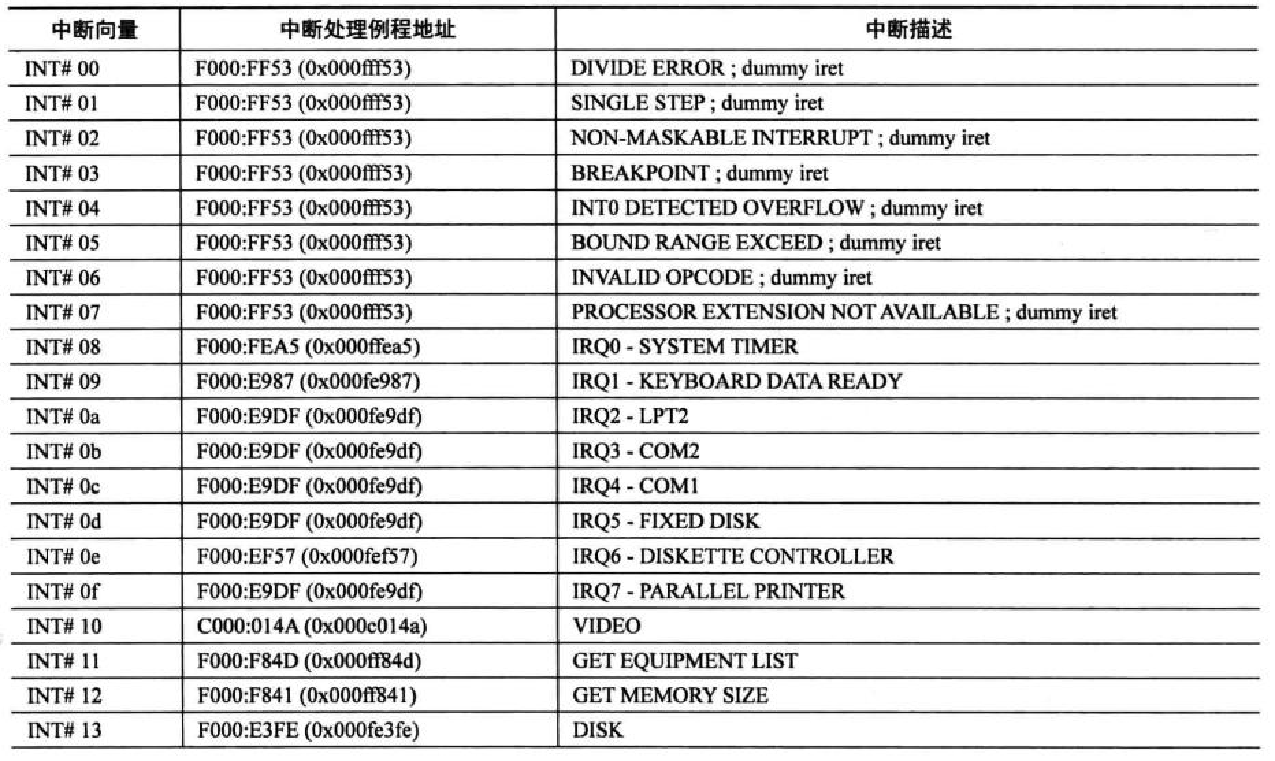
\includegraphics[width=15cm]{中断1}
  \caption{中断向量表1}
  \label{fig:itpt1}
\end{figure}
\begin{figure}[H]
  \centering
  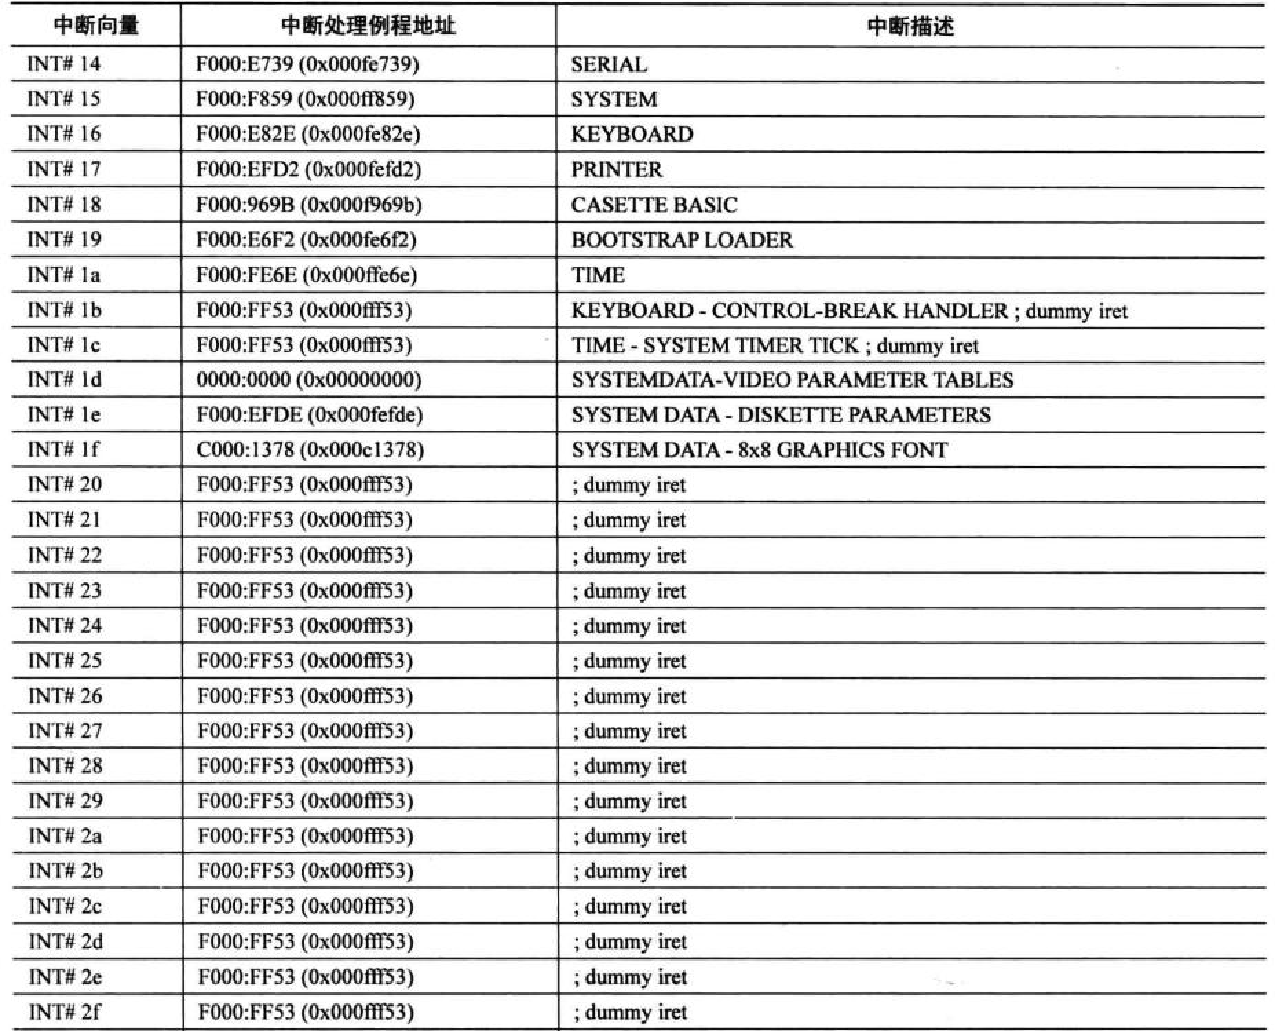
\includegraphics[width=15cm]{中断2}
  \caption{中断向量表2}
  \label{fig:itpt2}
\end{figure}
\begin{figure}[H]
  \centering
  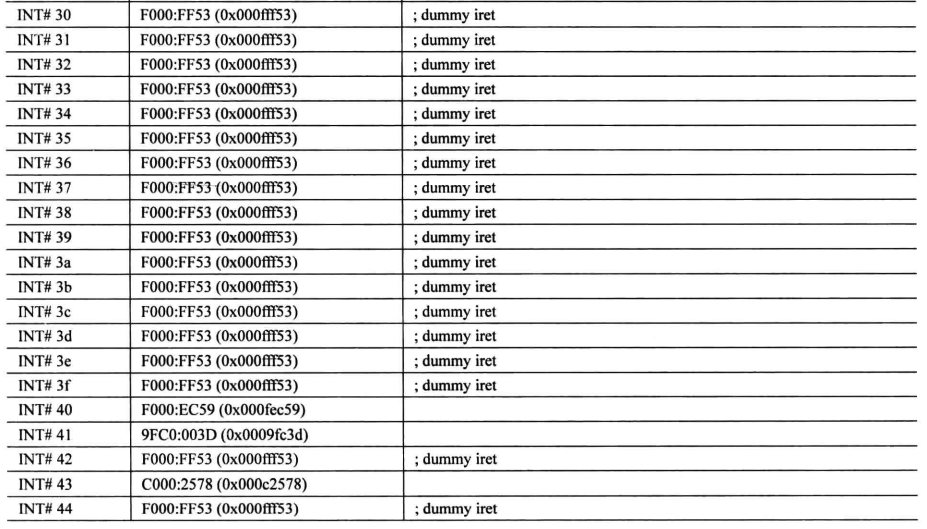
\includegraphics[width=15cm]{中断3}
  \caption{中断向量表3}
  \label{fig:itpt3}
\end{figure}
\begin{figure}[H]
  \centering
  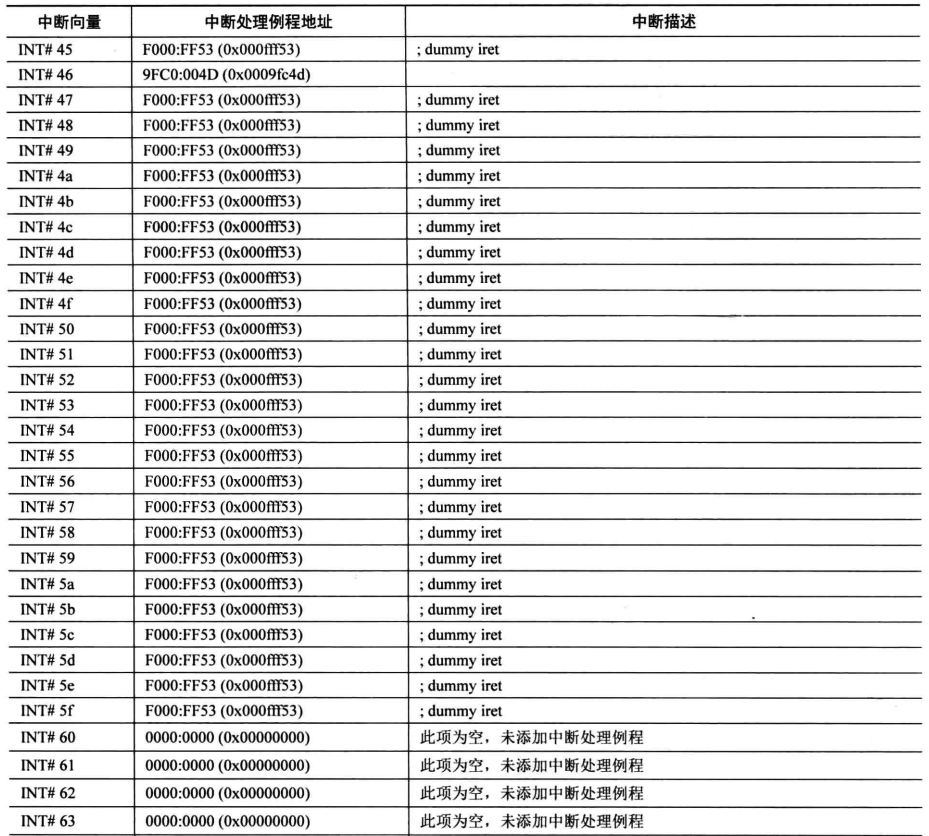
\includegraphics[width=15cm]{中断4}
  \caption{中断向量表4}
  \label{fig:itpt4}
\end{figure}
\begin{figure}[H]
  \centering
  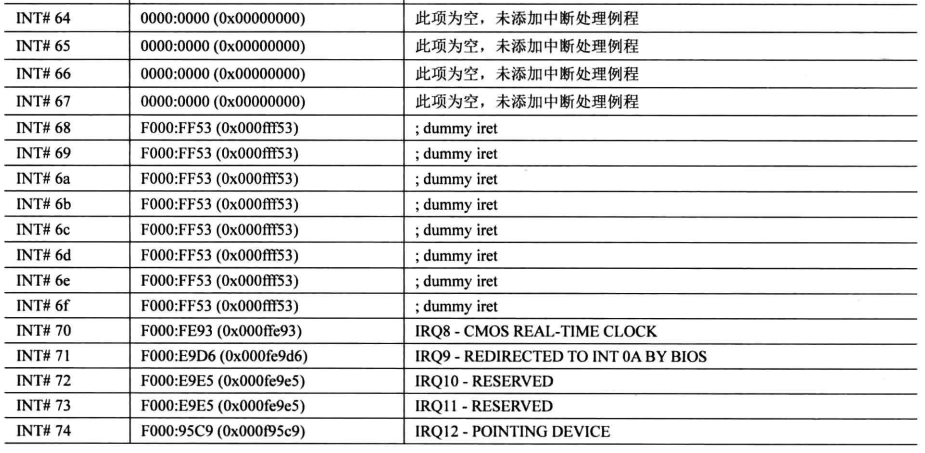
\includegraphics[width=15cm]{中断5}
  \caption{中断向量表5}
  \label{fig:itpt5}
\end{figure}
\begin{figure}[H]
  \centering
  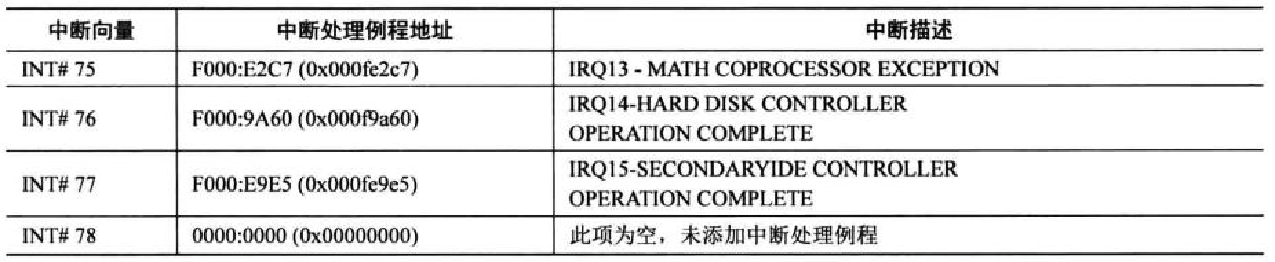
\includegraphics[width=15cm]{中断6}
  \caption{中断向量表6}
  \label{fig:itpt6}
\end{figure}

\section{键盘扫描码}
\label{sec:key}
\begin{figure}[H]
  \centering
  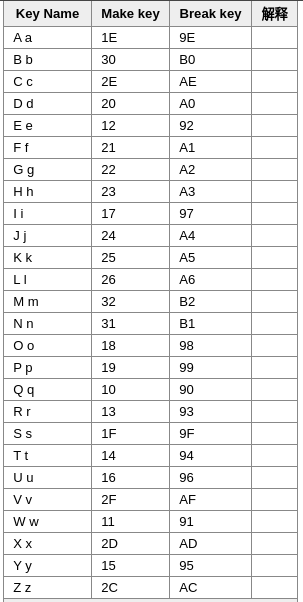
\includegraphics[width=12cm]{扫描码1}
  \caption{Scan code set 1}
  \label{fig:key1}
\end{figure}
\begin{figure}[H]
  \centering
  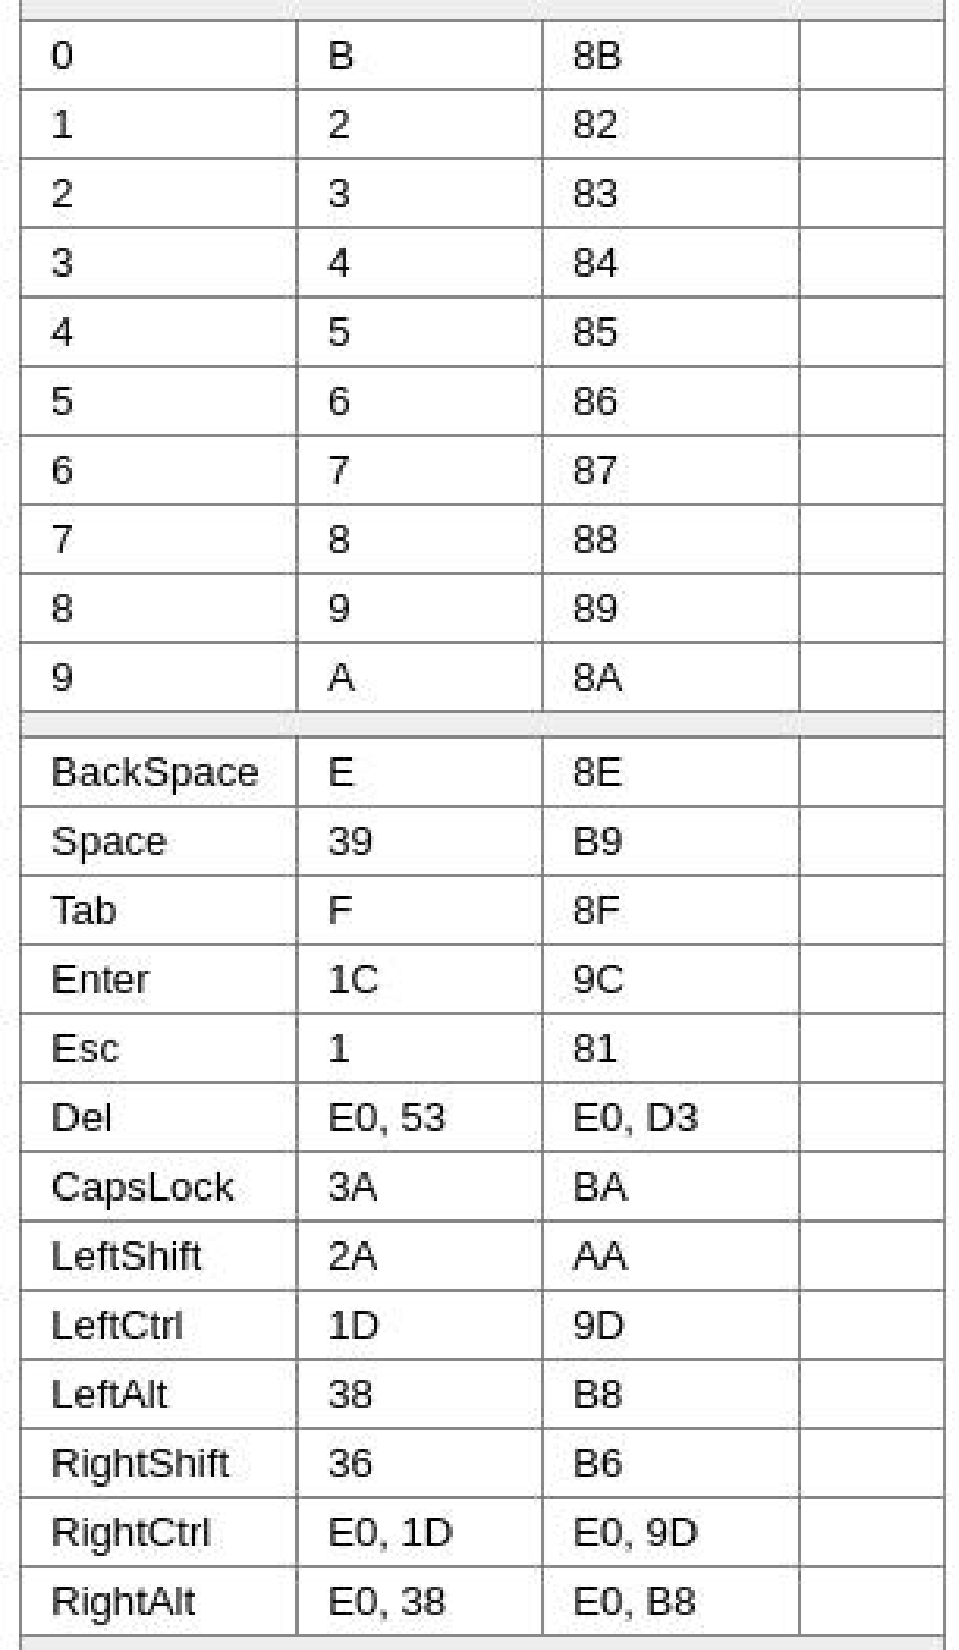
\includegraphics[width=12cm]{扫描码2}
  \caption{Scan code set 1}
  \label{fig:key2}
\end{figure}
\begin{figure}[H]
  \centering
  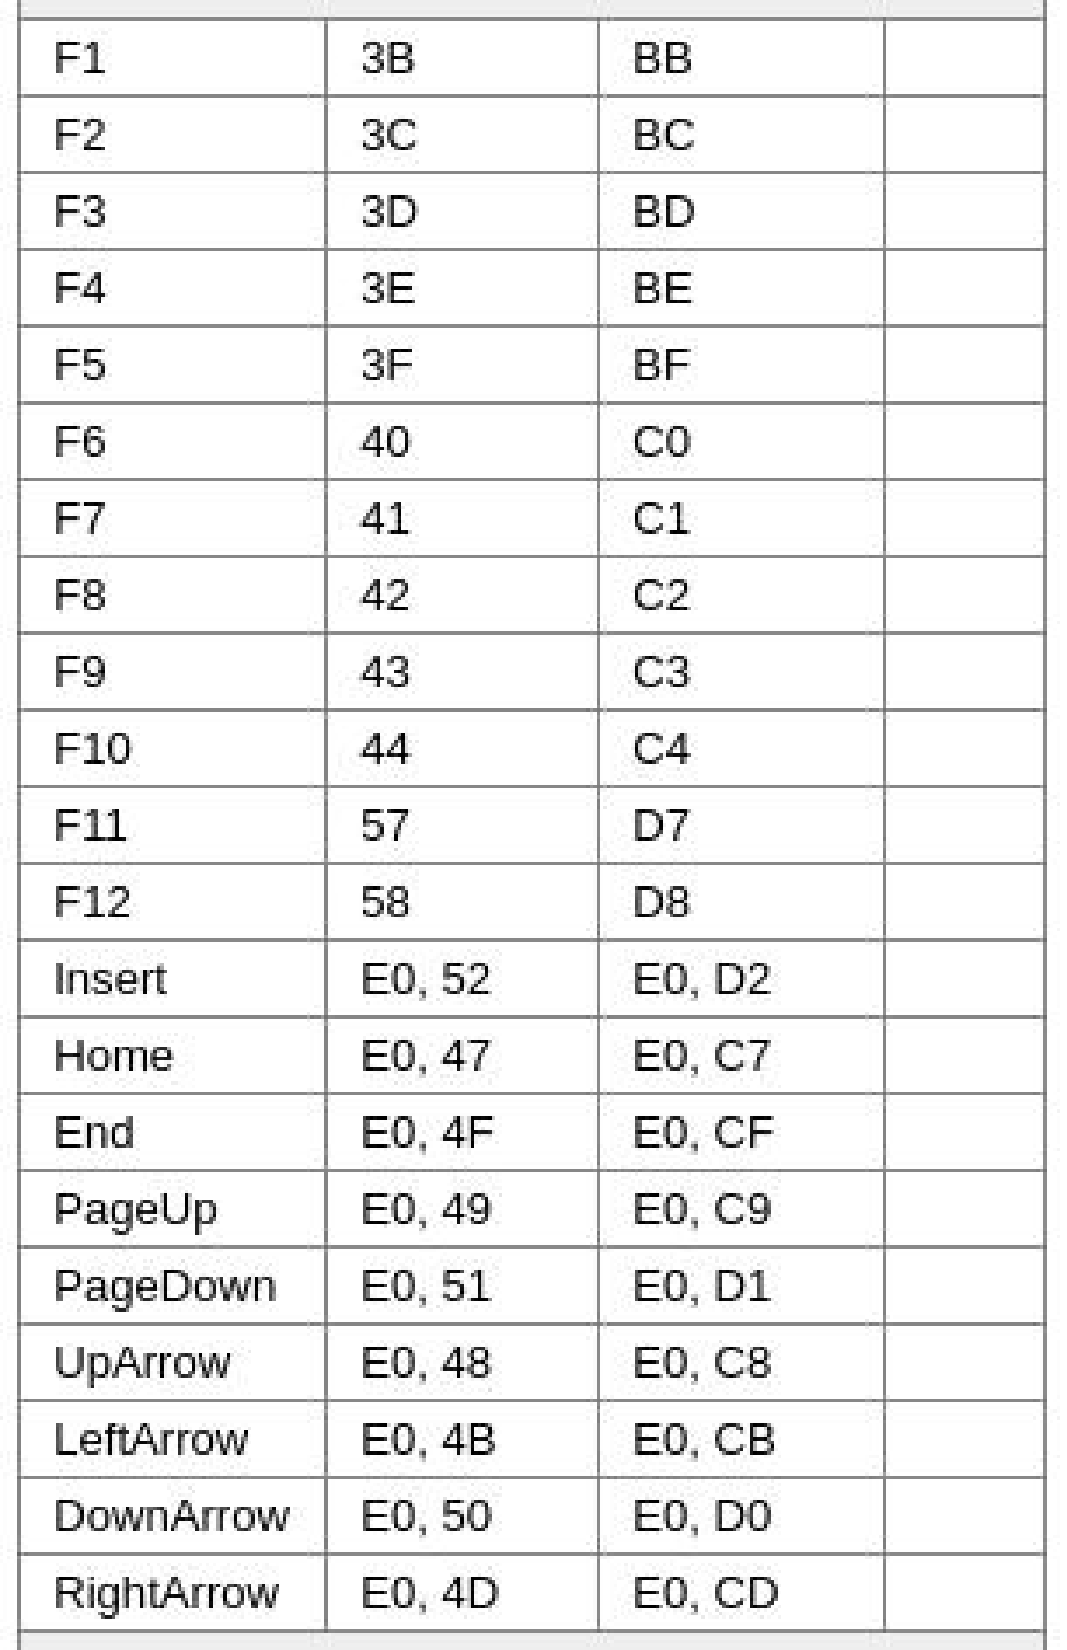
\includegraphics[width=12cm]{扫描码3}
  \caption{Scan code set 1}
  \label{fig:key3}
\end{figure}
\begin{figure}[H]
  \centering
  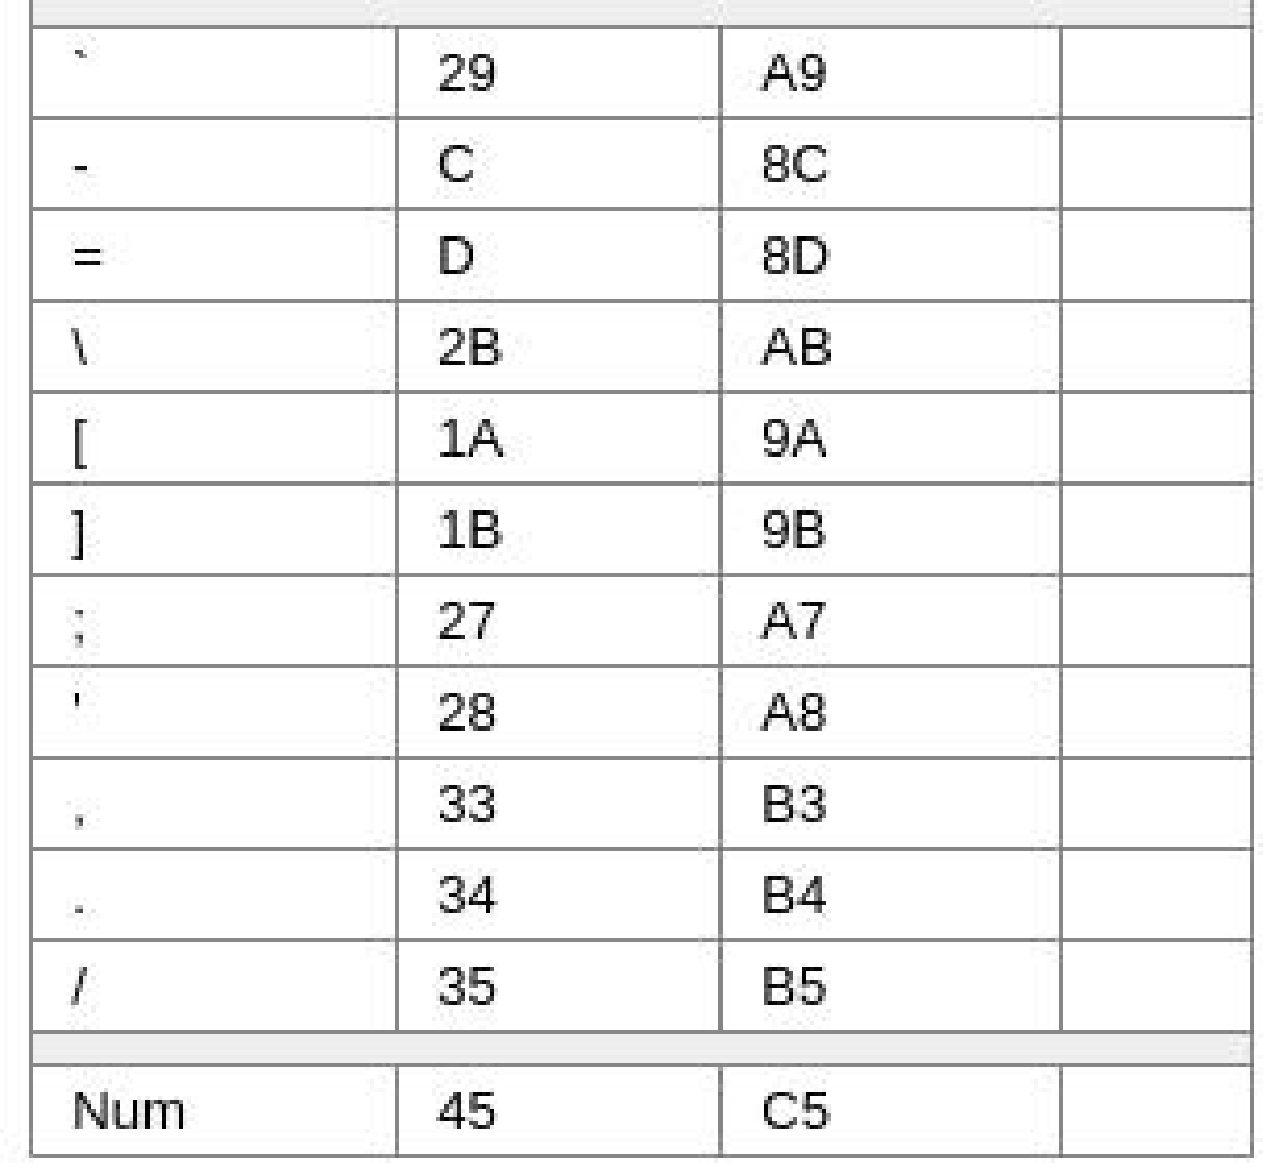
\includegraphics[width=12cm]{扫描码4}
  \caption{Scan code set 1}
  \label{fig:key4}
\end{figure}
%%% Local Variables:
%%% mode: latex
%%% TeX-master: "../thesis"
%%% End:
 %       │      │   ├── ch2.tex
%\include{chapters/ch8} %       │      │   ├── ch3.tex
%\include{chapters/ch9} %       │      │   └── ...
%\include{chapters/cha} %       │      ├── figs/
%\include{chapters/chb} %       │      │   ├── flowchart.pdf
%\include{chapters/chc} %       │      │   └── ...
%\include{chapters/chd} %       │      └── ...
%\include{chapters/che} %       └── src/
%\include{chapters/chf} %              ├── hello.c
%\include{chapters/chg} %              └── ...
%\include{chapters/chh} %%%

%%%%% appendix (参考文献、指导教师简介、鸣谢、附录)
\appendix % keep this line
\makebib % 参考文献

\begin{advisorInfo} % 指导教师简介
  王晓林,男,50岁,硕士,讲师,毕业于英国格林尼治大学,分布式计算系统专业。现任
  西南林业大学计信学院教师。执教Linux、操作系统、网络技术等方面的课程,有丰富的Linux教学和系统管理经验。
\end{advisorInfo}

\begin{acknowledgment} % 致谢
  首先我要感谢对我悉心指导和引导我走进LinuxOS世界的指导老师,王晓林老师,如果没有遇到他的
  话,我甚至可能不会接触Linux这个操作系统,感谢他在这方面给予了我很多帮助,在遇到很多Linux
  方面的问题是都是他帮助我解决了,因为有他所以我才能从一位Windows用户变到Linux用户然后再爱
  上Linux。其次,还要感谢两本书的作者,他们分别是《OrangeS:一个操作系统的实现》的作者于渊
  和《操作系统真相还原》的作者郑钢,如果没有他们写的这两本书的话,我的这次毕业设计将会困难
  重重,他们写的书给了我很多帮助,很多地方都解释的非常到位,基本上从头到尾跟着做一遍下来的
  话都是能够理解的。最后还要感谢期间帮助过我的朋友、同学们,如果没有他们的鼓励和支持的话也
  许我也早就放弃了,感谢大家对我的帮助。
\end{acknowledgment}

%%%%% 附录章节
\singlespacing
%\chapter{不足与展望}
通过对Linux操作系统的学习和本次毕业设计实践,让我对计算机的工作原理、
操作系统的概念、和系统编程有了更加深刻的了解。不足之处有以下几点:
\begin{enumerate}
\item 实现的功能较少,仅有一些简单的对文件的操作。
\item 我觉得接触到的东西虽然已经说是底层的了,但并不是最底层的,像\texttt{nasm}、\texttt{gcc}、\texttt{ld}这些指令都
  是前人写好的,直接拿来用了,以后若是有时间定会研究一下由自己写的编译器来编译自己写的程序。
\item Tab自动补全的功能,我自己在日常使用中最常用的也就是这个键,这次没有实现还是挺遗憾的。
\item 网络相关的知识,虽然现在感觉离这个层面还很远,但感觉以后若是涉及到这方面的问题一定也
  会很有趣。
\end{enumerate}

基本上就是以上这些地方感觉要是有时间的话还是能够实现的,所以就带有一丝丝遗憾,由于要准备考
试以及一些其他原因,对这次毕业设计的时间其实很紧张,然后操作系统里的很多东西都是很底层的,
像汇编、和一些基础的C语言\cite{HD2008}学习起来就需要更多的时间去了解相关的知识,最后感觉也只是了解到了
一点皮毛,说实话也就是在别人铺好的路上走了一遍,用着别人提前写好的一些框架。

其实在最初定下要研究这个题目的时候,目标是想将显示PDF这些功能也加进去,最后能在我自己制作
的SheepOS进行论文答辩,那肯定是件非常有意义的事,但现实总比理想要残酷的多,感觉还差的很远
,以后还需要继续努力,加油。

%%% Local Variables:
%%% mode: latex
%%% TeX-master: "../thesis"
%%% End:

\chapter{相关代码}%
\section{MBR}
\label{fsec:mbr}
\inputminted{nasm}{./code/mbr.S}

\section{Rd Disk}
\label{fsec:loader_disk}
\inputminted{nasm}{./code/loader_disk.S}

\section{BIOS 0x15 interrupt}
\label{fsec:loader_15h}
\inputminted{nasm}{./code/loader_15h.S}

\section{Page}
\label{fsec:loader_page}
\inputminted{nasm}{./code/loader_page.S}

\section{Kernel init}
\label{fsec:kernel_init}
\inputminted{nasm}{./code/kernel_init.S}

\section{Print Put Char}
\label{fsec:put_char}
\inputminted{nasm}{./code/put_char.S}

\section{Print Put Int}
\label{fsec:put_int}
\inputminted{nasm}{./code/put_int.S}

\section{Interrupt}
\label{app:int_a}
\inputminted{nasm}{./code/int_a.S}

\section{Idt Table}
\label{app:int_b}
\inputminted{c}{./code/idt_b.c}

\section{keyboard}
\label{sec:keyb}
\inputminted{c}{./code/keyboard.c}

\section{process}
\label{sec:process}
\inputminted{c}{./code/process.c}

\section{Schedule}
\label{fsec:schedule}
\inputminted{c}{./code/schedule.c}

\section{File System}
\label{app:partitionformat}
\inputminted{c}{./code/fs_sys.c}

\section{File Create}
\label{app:filecreate}
\inputminted{c}{./code/fs_create.c}

\section{File Open/Close}
\label{app:fileopen}
\inputminted{c}{./code/fs_open.c}

\section{File Delete}
\label{app:filedel}
\inputminted{c}{./code/fs_del.c}

%%% Local Variables:
%%% mode: latex
%%% TeX-master: "../thesis"
%%% End:


\end{document} % 结束。不要动下面几行!

%%% Local Variables:
%%% mode: latex
%%% TeX-master: t
%%% TeX-master: t
%%% TeX-master: t
%%% End:

